\graphicspath{ {Figures/system_analysis/} }

\chapter{Ανάλυση και σχεδιασμός του συστήματος LifeDonor}\label{ch:Analysis of LifeDonor}
\section{Λειτουργικές απαιτήσεις}

	Οι απαιτήσεις ενός συστήματος αποτελούν τη βάση των συστημάτων λογισμικού. Ουσιαστικά, είναι η περιγραφή των υπηρεσιών που πρέπει να παρέχει ένα σύστημα λογισμικού και οι περιορισμοί υπό τους οποίους πρέπει αυτές να λειτουργούν. Διακρίνονται σε δύο βασικές κατηγορίες τις λειτουργικές απαιτήσεις (functional requirements) και τις μη λειτουργικές απαιτήσεις(non functional requirements). 
	
	Οι λειτουργικές απαιτήσεις προσδιορίζουν τα βασικά χαρακτηριστικά του συστήματος και την λειτουργία του από την άποψη του ίδιου του προϊόντος και των χρηστών του. Στον όρο λειτουργία του συστήματος συμπεριλαμβάνεται οι συνολικές είσοδοι, η συμπεριφορά και οι έξοδοι του συστήματος. Στο σύστημα που υλοποιούμε, οι λειτουργικές απαιτήσεις χρησιμοποιούνται για να περιγράψουν ειδικές λειτουργίες που καθορίζουν αυτά τα οποία αναμένουμε να πετύχει το σύστημα. Αν και αναφέρονται ως "απαιτήσεις", στην πραγματικότητα αποτελούν μια μορφή σχεδιασμού, υψηλού επιπέδου. Οι λειτουργικές απαιτήσεις συχνά προσδιορίζονται ως λειτουργικές προδιαγραφές,» και ο όρος περιγραφή αποτελεί συνώνυμο του σχεδιασμού. Οι λειτουργικές απαιτήσεις είναι ουσιαστικά το "τι" λειτουργία θέλουμε να επιτελεί το σύστημα, χωρίς να παρέχουμε καμία πληροφορία για το "πως".
	
	Οι μη λειτουργικές απαιτήσεις είναι οι απαιτήσεις που καθορίζουν τα κριτήρια που χρησιμοποιούνται για να κρίνουν την λειτουργία του συστήματος και κατά επέκταση  αν είναι επιτυχημένο ή όχι, για αυτό και συχνά αποκαλούνται και ιδιότητες του. Επεξεργάζονται τα χαρακτηριστικά απόδοσης του, και μπορούν επίσης να περιγράψουν τις πτυχές του συστήματος που δεν σχετίζονται με την εκτέλεση του, αλλά με την εξέλιξη του στο πέρασμα του χρόνου. Οι βασικές συνήθεις κατηγορίες των μη λειτουργικών απαιτήσεων σχετίζονται με την ασφάλεια( ασφαλή πρόσβαση σε δεδομένα αλλά και σε hardware), την απόδοση ( ορίζουν χαρακτηριστικά που έχουν να κάνουν με την ταχύτητα και την ανταπόκριση του συστήματος) και την επεκτασιμότητα (σχετίζονται με το μέγεθος του συστήματος). Γενικότερα, οι μη λειτουργικές απαιτήσεις καθορίζουν το πώς πρέπει να είναι ένα σύστημα, σε αντίθεση με τις λειτουργικές απαιτήσεις που καθορίζουν τι πρέπει να κάνει ένα σύστημα. Οι λειτουργικές απαιτήσεις ανήκουν στο κομμάτι σχεδιασμού και ανάλυσης του συστήματος ενώ οι μη λειτουργικές απαιτήσεις ανήκουν στο κομμάτι της αρχιτεκτονικής του συστήματος.
	
	\subsection{Λειτουργίες εφαρμογής (web, mobile)}
Οι χρήστες του συστήματος χωρίζονται σε τρεις μεγάλες ομάδες χρηστών.

		\begin{enumerate}

			\item Εθελοντές αιμοδότες
			\item Εγκεκριμένοι χρήστες/διαχειριστές των συστημάτων αιμοδοσίας
			\item Υπέρ-Διαχειριστές του συστήματος

		\end{enumerate}
		
		Οι εθελοντές αιμοδότες αποτελούν την βασική κατηγορία χρηστών καθώς πραγματοποιούν συνεχή και εκτεταμένη χρήση των υπηρεσιών του συστήματος, τόσο στο επίπεδο της εφαρμογής έξυπνου κινητού όσο και μέσω του web portal. Οι εγκεκριμένοι χρήστες/διαχειριστές των συστημάτων αιμοδοσίας χρησιμοποιούν αποκλειστικά το web portal το οποίο βρίσκεται στο υπολογιστικό νέφος για ολοκληρωμένη διαχείριση ενός πλήρους κύκλου αιμοδοσίας. Οι λειτουργίες που μπορεί να επιτελέσει κάθε ομάδα χρηστών καθώς και οι λειτουργικές απαιτήσεις του συστήματος αναλύονται με λεπτομέρειες στην συνέχεια.
		
		\subsubsection{Mobile} \label{sssec:functional_requirements_mobile}
			Επιγραμματικά, οι λειτουργικές απαιτήσεις της εφαρμογής έξυπνου κινητού είναι οι εξής:
			
			\begin{itemize}
				\item Δυνατότητα εγγραφής στο σύστημα ως εθελοντής αιμοδότης με χρήση του αριθμού μητρώου κοινωνικής ασφάλισης (Α.Μ.Κ.Α.).
				\item Δυνατότητα σύνδεσης στο σύστημα αν έχει πραγματοποιήσει ήδη έγγραφή στο παρελθόν.
				\item Δυνατότητα προβολής γεγονότων αιμοδοσίας.
				\item Δυνατότητα λήψης ειδοποιήσεων (push notifications) όταν δημιουργείται κάποιο νέο γεγονός αιμοδοσίας για το οποίο ο εθελοντής αιμοδότης πληρεί τα απαραίτητα κριτήρια.
				\item Δυνατότητα αποδοχής, απόρριψης ή αναβολής της ειδοποίησης για το γεγονός αιμοδοσίας.
				\item Δυνατότητα διαχείρισης ραντεβού για αιμοδοσία (δημιουργία νέου ραντεβού, μετάθεση , προβολή, ακύρωση).
				\item Δυνατότητα προσθήκης και συγχρονισμού των ραντεβού αιμοδοσίας στο ημερολογίου του χρήστη.
				\item Δυνατότητα ενημέρωσης σχετικά με το υπολειπόμενο διάστημα που πρέπει να παρέλθει ώστε ο εθελοντής να είναι σε θέση να συμμετέχει σε μία νέα αιμοδοσία.
				\item Δυνατότητα να κερδίσει πόντους και εμβλήματα βάση των αιμοδοσιών του (gamification system) και να τα μοιραστεί στα μέσα κοινωνικής δικτύωσης.
				\item Δυνατότητα να μοιραστεί και να δημοσιεύσει στοιχεία στα μέσα κοινωνικής δικτύωσης σε κάθε στάδιο της αιμοδοσίας.
				\item Δυνατότητα δημιουργίας έκκλησης για αίμα σε περίπτωση ανάγκης ατόμων του στενού κύκλου χρήστη και δημοσίευσης του στα μέσα κοινωνικής δικτύωσης.
				\item Δυνατότητα διαχείρισης προφίλ χρήστη.

			\end{itemize}

			\subsubsection{Web Portal} \label{sssec:functional_requirements_web}
			
				Το web portal που βρίσκεται στο υπολογιστικό νέφος χρησιμοποιείται από όλες τις ομάδες χρηστών. Όσον αφορά στους εθελοντές αιμοδότες ισχύουν οι ίδιες λειτουργικές απαιτήσεις όπως στην εφαρμογή του έξυπνου κινητού οι οποίες και αναλύθηκαν παραπάνω στο \ref{sssec:functional_requirements_mobile}. Όσον αφορά στους χρήστες/διαχειριστές των κέντρων αιμοδοσίας έχουμε τις παρακάτω λειτουργικές απαιτήσεις:
				
				\begin{itemize}
					\item Δημιουργία νέων γεγονότων αιμοδοσίας.
				%	\item Αποστολή ειδοποιήσεων στους εθελοντές αιμοδότες βάση των γεγονότων αιμοδοσίας, των αναγκών και των κριτηρίων αποδοχής.
					\item Προβολή στατιστικών ανά έτος σχετικά με τις ειδοποιήσεις που στάλθηκαν από το συγκεκριμένο κέντρο αιμοδοσίας και την ανταπόκριση των χρηστών (αποδοχή, απόρριψη, άνοιγμα ειδοποίησης, ολοκλήρωση αιμοδοσίας).
					\item Διαχείριση των ραντεβού για αιμοληψία.
					\item Διαχείριση του προφίλ του κέντρου αιμοδοσίας.
				%	\item Εισαγωγή δεδομένων από το τοπικό τους σύστημα στο κεντρικό σύστημα μας που βρίσκεται στο υπολογιστικό νέφος
					\item Δυνατότητα εγγραφής στο σύστημα νέου εθελοντή αιμοδότη.
					\item Δυνατότητα καταχώρησης της ολοκλήρωσης της αιμοδοσίας.
					\item Δυνατότητα ελέγχου τήρησης προϋποθέσεων καταλληλότητας εθελοντή αιμοδότη.
				\end{itemize}
				Όσον αφορά στους υπέρ-διαχειριστές του συστήματος έχουμε τις παρακάτω λειτουργικές απαιτήσεις:
				\begin{itemize}
					\item Δυνατότητα διαχείρισης λογαριασμών χρηστών.
					\item Προβολή στατιστικών για τους χρήστες του συστήματος.
				\end{itemize}

	
\section{Σενάρια χρήσης}

	Η διαδικασία της μοντελοποίησης, δηλαδή ο αναλυτικός σχεδιασμός ενός συστήματος, πριν από την υλοποίηση του είναι ένα πολύ βασικό στάδιο κατά την ανάπτυξη εφαρμογών. Ένα σύστημα μοντελοποιείται επιτυχώς όταν οι λειτουργικότητες του συστήματος έχουν περιγραφεί πλήρως και ορθώς, έχουν καλυφθεί οι ανάγκες των τελικών χρηστών και υποστηρίζεται η επεκτασιμότητα του συστήματος. 
	Η ενοποιημένη Γλώσσα Μοντελοποίησης (UML) είναι μια τυπική γλώσσα για τη σύνταξη λεπτομερών σχεδίων λογισμικού. Η UML μπορεί να χρησιμοποιηθεί για να απεικονίσει, να προσδιορίζει,να κατασκευάσει και να τεκμηριώσει τα προϊόντα του συστήματος εντάσεως λογισμικού.\cite{Booch2005}. Δεν αποτελεί απλώς έναν κατάλογο από διαγράμματα, αλλά είναι μια γλώσσα αναπαράστασης γνώσης. Αυτό συνεπάγεται ότι κάθε στοιχείο διαγράμματος, π.χ. κουτί, βέλος, κύκλος, ορθογώνιο κ.λ.π., υποστηρίζεται από συγκεκριμένους κανόνες σύνταξης και σημασιολογία.
	 Επιλέξαμε να μοντελοποιήσουμε το σύστημα μας με χρήση της γλώσσας UML για τους εξής λόγους:
	 
	 \begin{itemize}
	 \item Είναι ένα βιομηχανικό πρότυπο από τον διεθνή, ανοιχτό και μη κερδοσκοπικό οργανισμό εταιριών Object Management Group (OMG).
	 \item Η UML είναι χτισμένη πάνω σε θεμελιώσεις αντικειμενοστραφείς έννοιες, όπως η κλάση, με αποτέλεσμα να υποστηρίζει καλύτερα την ανάπτυξη και τον σχεδιασμό του αντικειμενοστραφούς λογισμικού.
	 \item Δίνει έμφαση στην ανάλυση των σεναρίων χρήσης, το οποίο είναι ένα πολύτιμο εργαλείο για την παρακολούθηση των σταδίων μιας διαδικασίας από την οπτική γωνία του χρήστη.
	 \item Δίνει στον σχεδιαστή την δυνατότητα να παρουσιάσει όσο λεπτομερώς επιθυμεί αυτός τις περιγραφές του συστήματος.
	 \item Τμηματοποιεί τον σχεδιασμό του συστήματος με αποτέλεσμα να αυξάνεται η επεκτασιμότητα του.
\end{itemize}	 

	Η UML 2.0 ορίζει δεκατρείς τύπους διαγραμμάτων, τα οποία μπορούν να χωριστούν σε δύο βασικές κατηγορίες:
	
	\begin{itemize}
		\item Τα διαγράμματα στατικής δομής, τα οποία δείχνουν τα πράγματα τα οποία απαρτίζουν το σύστημα που μοντελοποιείται και δεν αλλάζουν στο πέρασμα του χρόνου, για παράδειγμα τις κλάσεις, τα αντικείμενα κλπ. Στα διαγράμματα δομής ανήκουν: τα διαγράμματα κλάσεων, τα διαγράμματα αντικειμένων, τα ψηφιδικά διαγράμματα, τα διαγράμματα σύνθετης δομής, τα διαγράμματα πακέτου και τα διαγράμματα διάταξης.
		
		\item Τα διαγράμματα συμπεριφοράς, τα οποία δίνουν έμφαση στο τι πρέπει να γίνει στο σύστημα που μοντελοποιούμε, όπως τις αλληλεπιδράσεις με τους χρήστες, τις διάφορες καταστάσεις του συστήματος κλπ. Διαγράμματα συμπεριφοράς αποτελούν τα ακόλουθα: τα διαγράμματα χρήσης, τα διαγράμματα δραστηριότης, τα διαγράμματα καταστάσεων μηχανής, τα ακολουθιακά διαγράμματα, τα συνεργατικά διαγράμματα και τα διαγράμματα χρονισμού.
	\end{itemize}
	
Κάθε ένα από τα παραπάνω διαγράμματα βλέπει το σύστημα από μια διαφορετική οπτική γωνία, π.χ. τα διαγράμματα χρήσης δείχνουν πώς οι χρήστες αλληλεπιδρούν με το σύστημα, τα διαγράμματα κλάσης δείχνουν τις κλάσεις του συστήματος και τις σχέσεις μεταξύ τους κλπ.
	
		Η πρακτική της ανάλυσης με σενάρια χρήσης τυποποιήθηκε για πρώτη φορά από τον Jacobson το 1994, ο οποίος περιέγραψε το σενάριο χρήσης σαν "μία σειρά από συναλλαγές που σχετίζονται ως προς την συμπεριφορά και εκτελούνται από έναν δράστη που βρίσκεται σε επικοινωνία με το σύστημα με σκοπό την παροχή κάποιας μετρήσιμης αξίας στον δράστη" \cite{Jacobson} . Ένα σενάριο χρήσης είναι μία συλλογή από πιθανά σενάρια μεταξύ του συστήματος και των εξωτερικών του δραστών. Κάθε σενάριο χρήσης χαρακτηρίζεται από τον στόχο που έχει ο κύριος δράστης του. Ο στόχος αυτός μπορεί να επιτευχθεί ή όχι. Τα σενάρια χρήσης αποτελούν ένα πολύ διαδεδομένο και πολύτιμο εργαλείο για την πλήρη αποτύπωση των λειτουργικών απαιτήσεων του συστήματος. Οι λειτουργικές απαιτήσεις μπορούν να εκφραστούν είτε με μορφή κειμένου, είτε με μορφή πίνακα. Επιλέξαμε να χρησιμοποιήσουμε την μορφή πίνακα, καθώς έχει πιο αυστηρή δομή με αποτέλεσμα να μειώνονται οι ασυνέπειες και οι περιττές πληροφορίες. \cite{Cockburn2000} και πιο συγκεκριμένα την μονή στήλη πρότυπο \cite{Cockburn2000} :
 
 
\begin{table}[H]
	\begin{center}
	    \begin{tabular}{|p{\dimexpr \linewidth-2\tabcolsep}|}
	    \hline
	    \rowcolor{grayy}
	    \textbf{Όνομα σεναρίου χρήσης}
	    \\ \hline    
	    Ο τίτλος του σεναρίου χρήσης, που συνήθως είναι ένα μία πρόταση που περιγράφει τον στόχο του κύριου δράστη.
	    \\ \hline
	    \rowcolor{grayy}
	    \textbf{Στόχος}
	    \\ \hline
 Μία μεγαλύτερη δήλωση η οποία περιγράφει τον στόχο του σεναρίου χρήσης με περισσότερες λεπτομέρειες.
	    \\ \hline
	    \rowcolor{grayy}
	    \textbf{Λεπτομέρειες}
	    \\ \hline
		\textbf{Δράστης:} Είναι οι δράστες που έχουν ως στόχο αυτόν που περιγράφεται από το σενάριο χρήσης.
		\\ \hline
		\textbf{Προϋποθέσεις:} Αυτά που ισχύουν πριν ξεκινήσει να εκτελείται το σενάριο χρήσης. Εφόσον είναι γνωστό ότι μια συνθήκη είναι αληθής, δεν θα ελεγχθεί ξανά κατά την διάρκεια εκτέλεσης του σεναρίου χρήσης. 
		\\ \hline
		\textbf{Ενέργεια ενεργοποίησης:} Καθορίζει ποιο γεγονός εκκινεί το σενάριο χρήσης. Η ενέργεια εκκίνησης αποτελεί το πρώτο βήμα του σεναρίου χρήσης. 
		\\ \hline
		\rowcolor{grayy}    
	    \textbf{Ροή γεγονότων}
	    \\ \hline
		\textbf{Κύρια ροή γεγονότων:}
		Η κύρια ροή γεγονότων περιγράφει την περίπτωση που όλα βαίνουν αισίως. Είναι μια σειρά από αριθμημένα βήματα, όπου το κάθε βήμα είναι μία ρητή εντολή- μετάβαση.
		\\ \hline
		\textbf{Επεκτάσεις:} 
Οι επεκτάσεις περιγράφουν τι μπορεί να συμβεί και με διαφορετικό τρόπο κατά την διάρκεια εκτέλεσης του επιτυχημένου σεναρίου. Μπορούν να οδηγήσουν σε επιτυχία ή σε αποτυχίες. Κάθε επέκταση αποτελείται από δύο διαφορετικά μέρη:
 \begin{itemize}
 \item Τις προϋποθέσεις κάτω από τις οποίες το σύστημα υιοθετεί μία διαφορετική συμπεριφορά. Μετά από αυτές τοποθετείται μία άνω και κάτω τελεία (:).
 \item Ο χειρισμός της επέκτασης που είναι μία ακολουθία από βήματα που απαιτούνται λόγω των προϋποθέσεων που υπάρχουν.
 \end{itemize}
		\\ \hline
		\textbf{Παραλλαγές:}
		 Οι παραλλαγές κάποιου βήματος από το επιτυχημένο σενάριο υπάρχουν επειδή ενώ αυτό που συμβαίνει σε κάποιο βήμα είναι πάντα το ίδιο υπάρχουν πολλοί τρόποι να το κάνουμε.
		 \\ \hline

	    \end{tabular}
	    \caption{Σενάριο χρήσης εγγραφής αιμοδότη}
		\label{tab:use_case_sample_table}
	\end{center}
\end{table}
 

 
	\subsubsection{Εφαρμογή}
	
	Θα αναπτύξουμε αρχικά τα σενάρια χρήσης της εφαρμογής.
	
- Σενάριο εγγραφής στο σύστημα ως εθελοντής αιμοδότης με χρήση του αριθμού μητρώου κοινωνικής ασφάλισης (Α.Μ.Κ.Α.).
\\*
\begin{table}[H]
	\begin{center}
	    \begin{tabular}{|p{\dimexpr \linewidth-2\tabcolsep}|}
	    \hline
	    \rowcolor{grayy}
	    \textbf{Όνομα σεναρίου χρήσης}
	    \\ \hline    
	    Εγγραφή στο σύστημα.
	    \\ \hline
	    \rowcolor{grayy}
	    \textbf{Στόχος}
	    \\ \hline
	   Ο χρήστης εισάγει τα προσωπικά του δεδομένα με σκοπό να δημιουργήσει το προσωπικό του μοναδικό αιμοδοτικό προφίλ.
	    \\ \hline
	    \rowcolor{grayy}
	    \textbf{Λεπτομέρειες}
	    \\ \hline
		\textbf{Δράστης:} Εθελοντής αιμοδότης.
		\\*
		\textbf{Προϋποθέσεις:} Να διαθέτει αριθμό ΑΜΚΑ.
		\\*
		\textbf{Ενέργεια ενεργοποίησης:} Μετάβαση στην sign up φόρμα
		\\ \hline
		\rowcolor{grayy}    
	    \textbf{Ροή γεγονότων}
	    \\* 
		\textbf{Κύρια ροή γεγονότων:}
		\begin{enumerate}
			\item	Ο χρήστης πηγαίνει στην επιλογή sign up και εισάγει το ΑΜΚΑ του.
			\item Στην συνέχεια συμπληρώνει την sign up φόρμα και επιλέγει ολοκλήρωση εγγραφής.
			\item Το σύστημα δημιουργεί ένα μοναδικό προφίλ για τον χρήστη, το οποίο εισάγει στην βάση δεδομένων του.
			\item Ο χρήστης ανακατευθύνεται στην αρχική σελίδα 
		\end{enumerate}
		\\ \hline
		\textbf{Επεκτάσεις:} 
		\begin{enumerate}
			\item	Ο χρήστης εισάγει ΑΜΚΑ για το οποίο έχει ήδη δημιουργηθεί κάποιο προφίλ.
			\item Το σύστημα τον ενημερώνει και τον καθοδηγεί ώστε να ανακτήσει τα στοιχεία του.
		\end{enumerate}
		\\*
		\\ \hline
	    \end{tabular}
	    \caption{Σενάριο χρήσης εγγραφής αιμοδότη}
		\label{tab:blood_donor_register}
	\end{center}
\end{table}

- Σύνδεση στο σύστημα αν έχει πραγματοποιήσει ήδη έγγραφή στο παρελθόν.
\\*
\begin{table}[H]	
	\begin{center}
	    \begin{tabular}{|p{\dimexpr \linewidth-2\tabcolsep}|}
	    \hline
	    \rowcolor{grayy}
	    \textbf{Όνομα σεναρίου χρήσης}
	    \\ \hline    
	    Σύνδεση στο σύστημα.
	     \\ \hline
	    \rowcolor{grayy}
	    \textbf{\textbf{Στόχος}}
	    \\ \hline
		Ο χρήστης εισάγει τα στοιχεία του ώστε να μεταφερθεί στον προσωπικό του λογαριασμό.
	    \\ \hline
	    \rowcolor{grayy}
	    \textbf{Λεπτομέρειες}
	    \\ \hline
		\textbf{Δράστης:} Εθελοντής αιμοδότης.
		\\*
		\textbf{Προϋποθέσεις:} Ο χρήστης πρέπει να είναι ήδη εγγεγραμμένος στο σύστημα.
		\\*
		\textbf{Ενέργεια ενεργοποίησης:} Μετάβαση στην sign in φόρμα.
		\\ \hline
		\rowcolor{grayy}    
	    \textbf{Ροή γεγονότων}
	    \\* 
		\textbf{Κύρια ροή γεγονότων:}
		\begin{enumerate}
			\item	Ο χρήστης εισάγει τα στοιχεία του και επιλέγει να συνδεθεί με το σύστημα.
			\item Το σύστημα αποκρίνεται θετικά αν υπάρχει εγγεγραμμένος  χρήστης με αυτά τα στοιχειά στην βάση δεδομένων του συστήματος, αλλιώς απαγορεύει
		την είσοδο στον χρήστη και τυπώνει το αντίστοιχο μήνυμα λάθους.
			\item	Ο χρήστης κατευθύνεται είτε στον προσωπικό του λογαριασμό (σωστή εισαγωγή στοιχειών) είτε του ζητείται να ξαναπροσπαθήσει να εισάγει τα σωστά στοιχεία στην sign in φόρμα.
		\end{enumerate}
		\\ \hline
		\textbf{Επεκτάσεις:}
		\\ \hline
		\begin{itemize}
		\item Ο χρήστης εισάγει μη έγκυρης  μορφής όνομα χρήστη ή κωδικό και επιλέγει να συνδεθεί με το σύστημα.
		\item Το σύστημα εμφανίζει μήνυμα λάθους, χωρίς να επικοινωνήσει με την βάση δεδομένων για ταυτοποίηση.
		\item Το σύστημα αναπροβάλει την φόρμα με μήνυμα οδηγιών στον χρήστη.
		\end{itemize}
	    \end{tabular}
	    \caption{Σενάριο χρήσης σύνδεσης στο σύστημα}
	    \label{tab:user_sign_in} 	
	\end{center}
\end{table}

- Προβολή  γεγονότων αιμοδοσίας.
\\*
\begin{table}[H]	
	\begin{center}
	    \begin{tabular}{|p{\dimexpr \linewidth-2\tabcolsep}|}
	    \hline
	    \rowcolor{grayy}
	    \textbf{Όνομα σεναρίου χρήσης}
	    \\ \hline    
	    Προβολή γεγονότων αιμοδοσίας
	     \\ \hline
	    \rowcolor{grayy}
	    \textbf{\textbf{Στόχος}}
	    \\ \hline
	    	Ο χρήστης θέλει να μπαίνει στην εφαρμογή και να βλέπει όλα τα ενεργά γεγονότα αιμοδοσίας, ταξινομημένα ανά την προτίμηση του(απόσταση, εναπομείνασες ημέρες κλπ) καθώς και τις απαραίτητες πληροφορίες για αυτά (τοποθεσία διεξαγωγής, ημερομηνίες, ομάδα αίματος κλπ)
	    \\ \hline
	    \rowcolor{grayy}
	    \textbf{Λεπτομέρειες}
	    \\ \hline
		\textbf{Δράστης:} Εθελοντής αιμοδότης.
		\\*
		\textbf{Προϋποθέσεις:} Ο χρήστης πρέπει να είναι ήδη εγγεγραμμένος στο σύστημα.
		\\*
		\textbf{Ενέργεια ενεργοποίησης:} Επιλογή της καρτέλας "Γεγονότα αιμοδοσίας".
	    \\ \hline
		\rowcolor{grayy}    
	    \textbf{Ροή γεγονότων}
	    \\ \hline
		\textbf{Κύρια ροή γεγονότων:}
		\begin{enumerate}
			\item	Ο χρήστης επιλέγει την καρτέλα "Γεγονότα αιμοδοσίας".
			\item Το σύστημα φορτώνει από την βάση δεδομένων και την προσωρινή μνήμη τα γεγονότα αιμοδοσίας.
			\item Ο χρήστης επιλέγει και αλλάζει την σειρά ως προς την οποία εμφανίζονται τα γεγονότα ανάλογα με κάποιο κριτήριο.
		\end{enumerate}
				\\ \hline
		\textbf{Επεκτάσεις:}
		   \\ \hline
	    \end{tabular}
	    \caption{Σενάριο χρήσης προβολής γεγονότων αιμοδοσίας}
	    \label{tab:blood_donation_events_show} 
	\end{center}
\end{table}

-Λήψης ειδοποιήσεων (push notifications) όταν δημιουργείται κάποιο νέο γεγονός αιμοδοσίας για το οποίο ο εθελοντής αιμοδότης πληρεί τα απαραίτητα κριτήρια.
\\*
\begin{table}[H]
	\begin{center}
	    \begin{tabular}{|p{\dimexpr \linewidth-2\tabcolsep}|}
	    \hline
	    \rowcolor{grayy}
	    \textbf{Όνομα σεναρίου χρήσης}
	    \\ \hline    
	     Λήψη ειδοποιήσεων (push notifications).
	     \\ \hline
	    \rowcolor{grayy}
	    \textbf{\textbf{Στόχος}}
	    \\ \hline
	 	 Ο εθελοντής αιμοδότης να μπορεί να λαμβάνει ειδοποιήσεις από το σύστημα σχετικά με ενεργές αιμοδοσίες. 
	    \\ \hline
	    \rowcolor{grayy}
	    \textbf{Λεπτομέρειες}
	    \\ \hline
		\textbf{Δράστης:} Εθελοντής αιμοδότης.
		\\*
		\textbf{Προϋποθέσεις:} Ο χρήστης πρέπει να είναι ήδη εγγεγραμμένος στο σύστημα.
		\\*
		\textbf{Ενέργεια ενεργοποίησης:} Δημιουργία νέου γεγονότος αιμοδοσίας.
		\\ \hline
		\rowcolor{grayy}    
	    \textbf{Ροή γεγονότων}
	    \\ \hline
		\textbf{Κύρια ροή γεγονότων:}
		\begin{enumerate}
			\item	Δημιουργείται ένα νέο συμβάν αιμοδοσίας.
			\item Το σύστημα με βάση το business model του αποφαίνεται αν ο χρήστης είναι σε θέση ή όχι να συμμετάσχει στην αιμοδοσία.
			\item Το σύστημα με βάση το αποτέλεσμα του προηγούμενου βήματος στέλνει ή όχι ειδοποίηση στον χρήστη.
			\item Ο χρήστης βλέπει την ειδοποίηση στο κινητό του.
		\end{enumerate}
				\\ \hline
		\textbf{Επεκτάσεις:}
		   \\ \hline
	    \end{tabular}
	    \caption{Σενάριο χρήσης λήψης ειδοποιήσεων}
	    \label{tab:receive_push_notifications} 
	\end{center}
\end{table}

-Αποδοχή, απόρριψη ή αναβολή της ειδοποίησης για το γεγονός αιμοδοσίας.
\\*
\begin{table}[H]
	\begin{center}
	    \begin{tabular}{|p{\dimexpr \linewidth-2\tabcolsep}|}
	    \hline
	    \rowcolor{grayy}
	    \textbf{Όνομα σεναρίου χρήσης}
	    \\ \hline    
	     Διαχείριση ειδοποιήσεων (push notifications).
	     \\ \hline
	    \rowcolor{grayy}
	    \textbf{\textbf{Στόχος}}
	    \\ \hline
	 	 Ο εθελοντής αιμοδότης να μπορεί να διαχειρίζεται αποτελεσματικά τις ειδοποιήσεις από το σύστημα σχετικά με ενεργές αιμοδοσίες, είτε πατώντας αποδοχή,  είτε απορρίπτοντας τες, είτε αναβάλλοντας τες.
	    \\ \hline
	    \rowcolor{grayy}
	    \textbf{Λεπτομέρειες}
	    \\ \hline
		\textbf{Δράστης:} Εθελοντής αιμοδότης.
		\\*
		\textbf{Προϋποθέσεις:} Ο χρήστης πρέπει να είναι ήδη εγγεγραμμένος στο σύστημα.
		\\*
		\textbf{Ενέργεια ενεργοποίησης:} Λήψη νέας ειδοποίησης (push notification).
		\\ \hline
		\rowcolor{grayy}    
	    \textbf{Ροή γεγονότων}
	    \\ \hline
		\textbf{Κύρια ροή γεγονότων:}
		\begin{enumerate}
		
			\item	Λήψη ειδοποίησης από το σύστημα για νέο γεγονός αιμοδοσίας.
			\item  Ο χρήστης επιλέγει μία από τις εξής ενέργειές: αποδοχή, απόρριψη, αναβολή.
			\item Το σύστημα αν ο χρήστης επιλέξει αποδοχή μεταφέρει το γεγονός στην λίστα με τα γεγονότα αιμοδοσίας που έχει αποδεχτεί ο χρήστης, αν επιλέξει απόρριψη μεταφέρει το γεγονός στην λίστα με τα γεγονότα που έχει απορρίψει, αλλιώς προγραμματίζει εκ νέου την αποστολή υπενθύμισης.

		\end{enumerate}
		\\ \hline
		\textbf{Επεκτάσεις:}
		   \\ \hline
	    \end{tabular}
	    \caption{Σενάριο χρήσης διαχείρισης ειδοποιήσεων}
	    \label{tab:manage_notifcations} 
	\end{center}		
\end{table}			
			
			
-Διαχείριση ραντεβού για αιμοδοσία (δημιουργία νέου ραντεβού, μετάθεση , προβολή, ακύρωση).
\\*

\begin{table}[H]
	\begin{center}
	    \begin{tabular}{|p{\dimexpr \linewidth-2\tabcolsep}|}
	    \hline
	    \rowcolor{grayy}
	    \textbf{Όνομα σεναρίου χρήσης}
	    \\ \hline    
	     Διαχείριση ραντεβού για αιμοδοσία.
	     \\ \hline
	    \rowcolor{grayy}
	    \textbf{\textbf{Στόχος}}
	    \\ \hline
	 	 Ο εθελοντής αιμοδότης να αλληλεπιδράσει με το σύστημα των ραντεβού, είτε δημιουργώντας ένα νέο ραντεβού για αιμοδοσία, είτε ακυρώνοντας ένα ήδη υπάρχον, είτε μεταθέτοντας την ημερομηνία ενός ραντεβού.
	    \\ \hline
	    \rowcolor{grayy}
	    \textbf{Λεπτομέρειες}
	    \\ \hline
		\textbf{Δράστης:} Εθελοντής αιμοδότης.
		\\*
		\textbf{Προϋποθέσεις:} Ο χρήστης πρέπει να έχει αποδεχτεί κάποιο γεγονός αιμοδοσίας.
		\\*
		\textbf{Ενέργεια ενεργοποίησης:} Αποδοχή κάποιου γεγονότος αιμοδοσίας ή μετάβαση στο ημερολόγιο.
		\\ \hline

		\rowcolor{grayy}    
	    \textbf{Ροή γεγονότων}
	    \\ \hline
		\textbf{Κύρια ροή γεγονότων:}
		\begin{enumerate}
			\item	 Ο χρήστης μεταφέρεται στο ημερολόγιο των ραντεβού, είτε αποδεχόμενος κάποιο γεγονός αιμοδοσίας, είτε με επιλογή της καρτέλας του ημερολογίου.
			\item  Ο χρήστης βλέπει τις διαθέσιμες ημερομηνίες και ώρες για ραντεβού για πραγματοποίηση αιμοδοσίας, με την επιλογή "Κλείσιμο ραντεβού", καθώς και τα ήδη υπάρχοντα ραντεβού, με τις επιλογές μετάθεση, διαγραφή.
			\item Το σύστημα ανάλογα με τις προηγούμενες ενέργειες του χρήστη κατοχυρώνει τις τελικές αλλαγές.
		\end{enumerate}
		\\ \hline
		\textbf{Επεκτάσεις:}
		   \\ \hline
	    \end{tabular}
	    \caption{Σενάριο χρήσης διαχείρισης ραντεβού αιμοδοσίας}
	    \label{tab:blood_donation_reservation_management} 
	\end{center}
\end{table}	
			
-Προσθήκη και συγχρονισμός των ραντεβού αιμοδοσίας στο ημερολόγιο του χρήστη.
\\*
\begin{table}[H]
	\begin{center}
	    \begin{tabular}{|p{\dimexpr \linewidth-2\tabcolsep}|}
	    \hline
	    \rowcolor{grayy}
	    \textbf{Όνομα σεναρίου χρήσης}
	    \\ \hline    
	    Προσθήκη των ραντεβού αιμοδοσίας στο ημερολόγιο του χρήστη.
	     \\ \hline
	    \rowcolor{grayy}
	    \textbf{\textbf{Στόχος}}
	    \\ \hline
	 	 Ο εθελοντής αιμοδότης να μπορεί να συγχρονίσει το σύστημα των ραντεβού του ολικού συστήματος αιμοδοσίας με το ημερολόγιο του, προσθέτοντας τα  ραντεβού αιμοδοσίας στις εφαρμογές ημερολογίου που χρησιμοποιεί(google calendar, calendar κλπ.)
	    \\ \hline
	    \rowcolor{grayy}
	    \textbf{Λεπτομέρειες}
	    \\ \hline
		\textbf{Δράστης:} Εθελοντής αιμοδότης.
		\\*
		\textbf{Προϋποθέσεις:} Ο χρήστης πρέπει να έχει κλείσει ραντεβού κάποιο γεγονός αιμοδοσίας.
		\\*
		\textbf{Ενέργεια ενεργοποίησης:} Άνοιγμα ραντεβού αιμοδοσίας  στο ημερολόγιο και επιλογή "προσθήκη στο ημερολόγιο μου".
	    \\ \hline
		\rowcolor{grayy}    
	    \textbf{Ροή γεγονότων}
	    \\ \hline
		\textbf{Κύρια ροή γεγονότων:}
		\begin{enumerate}
		\item	 Ο χρήστης μεταφέρεται στο ημερολόγιο των ραντεβού αιμοδοσίας της εφαρμογής και αφού ανοίξει κάποιο προγραμματισμένο ραντεβού επιλέγει το "προσθήκη στο ημερολόγιο μου".
		\item  Το σύστημα, εφόσον ο χρήστης το έχει εξουσιοδοτήσει με άδεια πρόσβασης στις εφαρμογές ημερολογίου του, συγχρονίζει τα ζητούμενα δεδομένα.
		\end{enumerate}
		\\ \hline
		\textbf{Επεκτάσεις:}
		   \\ \hline
		\begin{enumerate}
			\item Το σύστημα δεν έχει τις απαραίτητες άδειες για πρόσβαση στις εφαρμογές ημερολογίων του χρήστη.
			\item Το σύστημα αιτεί τις απαραίτητες άδειες από τον χρήστη.
			\item Το σύστημα εκκινεί την διαδικασία συγχρονισμού αν ο χρήστης του παραχωρήσει δικαιώματα πρόσβασης, αλλιώς εμφανίζει μήνυμα αποτυχίας.
		\end{enumerate}
		\\ \hline
	    \end{tabular}
	    \caption{Σενάριο χρήσης προσθήκης ραντεβού αιμοδοσίας στο ημερολόγιο}
	    \label{tab:add_blood_donation_to_calendar}
	\end{center}
\end{table}	
		
- Ενημέρωση σχετικά με το υπολειπόμενο διάστημα που πρέπει να παρέλθει ώστε ο εθελοντής να είναι σε θέση να συμμετέχει σε μία νέα αιμοδοσία.
\\*
\begin{table}[H]
	\begin{center}
	    \begin{tabular}{|p{\dimexpr \linewidth-2\tabcolsep}|}
	    \hline
	    \rowcolor{grayy}
	    \textbf{Όνομα σεναρίου χρήσης}
	    \\ \hline    
	     Ενημέρωση για το υπολειπόμενο διάστημα υποχρεωτικής αποχής του αιμοδότη.
	     \\ \hline
	    \rowcolor{grayy}
	    \textbf{\textbf{Στόχος}}
	    \\ \hline
	 	 Ο εθελοντής αιμοδότης να μπορεί να ενημερώνεται απλά και γρήγορα σχετικά με το διάστημα ου πρέπει να παρέλθει ώστε να είναι σε θέση να συμμετάσχει ξανά σε αιμοδοσία.
	    \\ \hline
	    \rowcolor{grayy}
	    \textbf{Λεπτομέρειες}
	    \\ \hline
		\textbf{Δράστης:} Εθελοντής αιμοδότης.
		\\*
		\textbf{Προϋποθέσεις:} Ο χρήστης πρέπει να έχει πραγματοποιήσει κάποια αιμοδοσία.
		\\*
		\textbf{Ενέργεια ενεργοποίησης:} Ο χρήστης μπαίνει στον προσωπικό του λογαριασμό στην εφαρμογή.
		\\ \hline
		\rowcolor{grayy}    
	    \textbf{Ροή γεγονότων}
	    \\ \hline
		\textbf{Κύρια ροή γεγονότων:}
		\begin{enumerate}
			\item	 Ο χρήστης μπαίνει στον προσωπικό του λογαριασμό στην εφαρμογή.
			\item  Το σύστημα με βάση τους κανονισμούς των αιμοδοτικών κέντρων για το απαιτούμενο διάστημα αποχής και την ημερομηνία τελευταίας αιμοδοσίας του εθελοντή, υπολογίζει τις υπολειπόμενες μέρες και τις εμφανίζει στον χρήστη.
		\end{enumerate}
		\\ \hline
		\textbf{Επεκτάσεις:}
		   \\ \hline
	    \end{tabular}
	    \caption{Σενάριο χρήσης ενημέρωσης για το υπολειπόμενο διάστημα υποχρεωτικής αποχής του αιμοδότη}
	    \label{tab:show_days_for_eligibility_to_donate} 
	\end{center}
\end{table}

-Προβολή πόντων και εμβλημάτων βάση των αιμοδοσιών του (gamification system) και κοινοποίηση στα μέσα κοινωνικής δικτύωσης.
\\*
\begin{table}[H]
	\begin{center}
	    \begin{tabular}{|p{\dimexpr \linewidth-2\tabcolsep}|}
	    \hline
	    \rowcolor{grayy}
	    \textbf{Όνομα σεναρίου χρήσης}
	    \\ \hline    
	     Gamification System
	     \\ \hline
	    \rowcolor{grayy}
	    \textbf{\textbf{Στόχος}}
	    \\ \hline
	 	 Ο εθελοντής αιμοδότης να μπορεί να κερδίζει πόντους και εμβλήματα βάση των αιμοδοσιών του και να κοινοποιεί στα μέσα κοινωνικής δικτύωσης.
	    \\ \hline
	    \rowcolor{grayy}
	    \textbf{Λεπτομέρειες}
	    \\ \hline
		\textbf{Δράστης:} Εθελοντής αιμοδότης.
		\\*
		\textbf{Προϋποθέσεις:} Ο χρήστης πρέπει να έχει πραγματοποιήσει αιμοδοσίες.
		\\*
		\textbf{Ενέργεια ενεργοποίησης:} Ο χρήστης επιλέγει την καρτέλα "Πόντοι και εμβλήματα".
		\\ \hline
		\rowcolor{grayy}    
	    \textbf{Ροή γεγονότων}
	    \\* 
		\textbf{Κύρια ροή γεγονότων:}
		\begin{enumerate}
		\item	 Ο χρήστης μπαίνει  στην καρτέλα "Πόντοι και εμβλήματα" της εφαρμογής.
		\item Ο χρήστης βλέπει τα εμβλήματα του και επιλέγει το έμβλημα που θέλει να μοιραστεί στα κοινωνικά δίκτυα.
		\item Το σύστημα, εφόσον ο χρήστης το έχει εξουσιοδοτήσει με άδεια πρόσβασης στους λογαριασμούς του ζητούμενα κοινωνικά δίκτυα, μοιράζεται τα δεδομένα.
		\end{enumerate}
		\\ \hline
		\textbf{Επεκτάσεις:}
		   \\ \hline
		\begin{enumerate}
			\item Το σύστημα δεν έχει τις απαραίτητες άδειες για πρόσβαση στους λογαριασμούς των κοινωνικών δικτύων του χρήστη,
			\item Το σύστημα αιτεί τις απαραίτητες άδειες από τον χρήστη.
			\item Το σύστημα εκκινεί την διαδικασία κοινοποίησης αν ο χρήστης του παραχωρήσει δικαιώματα πρόσβασης, αλλιώς εμφανίζει μήνυμα αποτυχίας.
		\end{enumerate}
		\\ \hline
	    \end{tabular}
	    \caption{Σενάριο χρήσης παιχνιδοποιήσης}
	    \label{tab:use_case_gamification} 
	\end{center}
\end{table}


-Δημοσίευση στοιχείων στα μέσα κοινωνικής δικτύωσης σε κάθε στάδιο της αιμοδοσίας.
\\*
\begin{table}[H]	
	\begin{center}
	    \begin{tabular}{|p{\dimexpr \linewidth-2\tabcolsep}|}
	    \hline
	    \rowcolor{grayy}
	    \textbf{Όνομα σεναρίου χρήσης}
	    \\ \hline    
	    Δημοσίευση στοιχείων από την αιμοδοσία στα μέσα κοινωνικής δικτύωσης.
	     \\ \hline
	    \rowcolor{grayy}
	   \textbf{Στόχος}
	    \\ \hline
	 	 Ο εθελοντής αιμοδότης να έχει την δυνατότητα σε διάφορα στάδια της αιμοδοσίας (αποδοχή αιτήματος, κλείσιμο ραντεβού) να κοινοποιεί δεδομένα στα μέσα κοινωνικής δικτύωσης.
	    \\ \hline
	    \rowcolor{grayy}
	    \textbf{Λεπτομέρειες}
	    \\ \hline
		\textbf{Δράστης:} Εθελοντής αιμοδότης.
		\\*
		\textbf{Προϋποθέσεις:} Ο χρήστης να έχει αποδεχτεί κάποια αιμοδοσία.
		\\*
		\textbf{Ενέργεια ενεργοποίησης:} Ο χρήστης επιλέγει να κάνει ανάρτηση μέσω της εφαρμογής στα μέσα κοινωνικής δικτύωσης.
		\\ \hline
		\rowcolor{grayy}    
	    \textbf{Ροή γεγονότων}
	    \\ \hline
		\textbf{Κύρια ροή γεγονότων:}
		\begin{enumerate}
		\item	 Ο χρήστης επιλέγει να κάνει ανάρτηση μέσω της εφαρμογής σε κάποιο στάδιο της διαδικασίας(αποδοχή, κλείσιμο ραντεβού, πραγματοποίηση αιμοδοσίας) .
		\item Ο χρήστης συμπληρώνει την περιγραφή της δημοσίευσης και επιλέγει τα μέσα κοινωνικής δικτύωσης στα οποία θέλει να γίνει η ανάρτηση.
	   \item Το σύστημα, εφόσον ο χρήστης το έχει εξουσιοδοτήσει με άδεια πρόσβασης στους λογαριασμούς του στα ζητούμενα κοινωνικά δίκτυα, μοιράζεται τα δεδομένα.
		\end{enumerate}
		\\*
		\textbf{Επεκτάσεις:}
		   \\ \hline
		\begin{enumerate}
			\item Το σύστημα δεν έχει τις απαραίτητες άδειες για πρόσβαση στους λογαριασμούς των κοινωνικών δικτύων του χρήστη,
			\item Το σύστημα αιτεί τις απαραίτητες άδειες από τον χρήστη.
			\item Το σύστημα εκκινεί την διαδικασία κοινοποίησης αν ο χρήστης του παραχωρήσει δικαιώματα πρόσβασης, αλλιώς εμφανίζει μήνυμα αποτυχίας.
		\end{enumerate}
		\\ \hline
	    \end{tabular}
	    \caption{Σενάριο χρήσης δημοσίευσης στοιχείων στα μέσα κοινωνικής δικτύωσης}
	    \label{tab:share_to_social_media} 
	\end{center}
\end{table}		

-Δημιουργία έκκλησης για αίμα σε περίπτωση ανάγκης ατόμων του στενού κύκλου χρήστη και δημοσίευσης του στα μέσα κοινωνικής δικτύωσης.
\\*
\begin{table}[H]
	\begin{center}
	    \begin{tabular}{|p{\dimexpr \linewidth-2\tabcolsep}|}
	    \hline
	    \rowcolor{grayy}
	    \textbf{Όνομα σεναρίου χρήσης}
	    \\ \hline    
	    Δημιουργία έκκλησης για αίμα.
	     \\ \hline
	    \rowcolor{grayy}
	    \textbf{\textbf{Στόχος}}
	    \\ \hline
	 	 Ο εθελοντής αιμοδότης να έχει την δυνατότητα να δημιουργήσει ένα νέο αίτημα για αιμοδοσία και να μπορεί να το δημοσιεύσει μέσω της εφαρμογής στα μέσα κοινωνικής δικτύωσης.
	    \\ \hline
	    \rowcolor{grayy}
	    \textbf{Λεπτομέρειες}
	    \\ \hline
		\textbf{Δράστης:} Εθελοντής αιμοδότης.
		\\*
		\textbf{Προϋποθέσεις:} Ο χρήστης να είναι εγγεγραμμένος στην εφαρμογή.
		\\*
		\textbf{Ενέργεια ενεργοποίησης:} Ο χρήστης επιλέγει την καρτέλα δημιουργία νέου γεγονότος αιμοδοσίας.
		\\ \hline
		\rowcolor{grayy}    
	    \textbf{Ροή γεγονότων}
	    \\ \hline
		\textbf{Κύρια ροή γεγονότων:}
		\begin{enumerate}
		\item	 Ο χρήστης επιλέγει να κάνει ανάρτηση μέσω της εφαρμογής  στα κοινωνικά δίκτυα..
		\item Ο χρήστης συμπληρώνει τα απαραίτητα πεδία στην φόρμα και επιλέγει δημιουργία νέου αιτήματος.
		\item Ο χρήστης επιλέγει κοινοποίηση του αιτήματος και τα μέσα κοινωνικής δικτύωσης στα οποία θέλει να γίνει η ανάρτηση.
	   \item Το σύστημα, εφόσον ο χρήστης το έχει εξουσιοδοτήσει με άδεια πρόσβασης στους λογαριασμούς του στα ζητούμενα κοινωνικά δίκτυα, μοιράζεται τα δεδομένα.
		\end{enumerate}
		\\*
		\textbf{Επεκτάσεις:}
		   \\ \hline
		\begin{enumerate}
			\item Το σύστημα δεν έχει τις απαραίτητες άδειες για πρόσβαση στους λογαριασμούς των κοινωνικών δικτύων του χρήστη,
			\item Το σύστημα αιτεί τις απαραίτητες άδειες από τον χρήστη.
			\item Το σύστημα εκκινεί την διαδικασία κοινοποίησης αν ο χρήστης του παραχωρήσει δικαιώματα πρόσβασης, αλλιώς εμφανίζει μήνυμα αποτυχίας.
		\end{enumerate}
		\\ \hline
	    \end{tabular}
	    \caption{Σενάριο χρήσης δημιουργίας έκκλησης για αίμα}
	    \label{tab:create_blood_donor_request} 
	\end{center}
\end{table}

-Διαχείριση προφίλ χρήστη.
\\*
\begin{table}[H]
	\begin{center}
	    \begin{tabular}{|p{\dimexpr \linewidth-2\tabcolsep}|}
	    \hline
	    \rowcolor{grayy}
	    \textbf{Όνομα σεναρίου χρήσης}
	    \\ \hline    
	    Διαχείριση προσωπικού προφίλ. 
	     \\ \hline
	    \rowcolor{grayy}
	    \textbf{\textbf{Στόχος}}
	    \\ \hline
	 	 Ο εθελοντής αιμοδότης να έχει την δυνατότητα να βλέπει και να επεξεργάζεται τα προσωπικά του στοιχεία.
	    \\ \hline
	    \rowcolor{grayy}
	    \textbf{Λεπτομέρειες}
	    \\ \hline
		\textbf{Δράστης:} Εθελοντής αιμοδότης.
		\\*
		\textbf{Προϋποθέσεις:} Ο χρήστης να είναι εγγεγραμμένος στην εφαρμογή.
		\\*
		\textbf{Ενέργεια ενεργοποίησης:} Ο χρήστης μεταβαίνει στις ρυθμίσεις του προσωπικού του λογαριασμού.
		\\ \hline
		\rowcolor{grayy}    
	    \textbf{Ροή γεγονότων}
	    \\ \hline
		\textbf{Κύρια ροή γεγονότων:}
		\begin{enumerate}
			\item	 Ο χρήστης μεταβαίνει στις ρυθμίσεις του προσωπικού του λογαριασμού.
			\item Τροποποιεί τα στοιχεία που επιθυμεί.
			\item Το σύστημα αποθηκεύει τις αλλαγές του χρήστη και ανανεώνει το προφίλ του, ώστε να βλέπει τα νέα δεδομένα.
		\end{enumerate}
		\\ \hline
		\textbf{Επεκτάσεις:}
		   \\ \hline
	    \end{tabular}
	    \caption{Σενάριο χρήσης διαχείρισης προσωπικού προφίλ}
	    \label{tab:profile_management}
	\end{center}
\end{table}	


 \subsubsection{Web portal}

Όσον αφορά στους χρήστες/διαχειριστές των κέντρων αιμοδοσίας έχουμε τα εξής σενάρια χρήσης:

-Δημιουργία νέων γεγονότων αιμοδοσίας.
\\*
\begin{table}[H]
	\begin{center}
	    \begin{tabular}{|p{\dimexpr \linewidth-2\tabcolsep}|}
	    \hline
	    \rowcolor{grayy}
	    \textbf{Όνομα σεναρίου χρήσης}
	    \\ \hline    
	    Δημιουργία γεγονότων αιμοδοσίας.
	     \\ \hline
	    \rowcolor{grayy}
	    \textbf{\textbf{Στόχος}}
	    \\ \hline
	 	 Ο εγκεκριμένος χρήστης/διαχειριστής να έχει την δυνατότητα να δημιουργήσει ένα νέο γεγονός αιμοδοσίας και να το καταχωρήσει στο σύστημα ώστε να ειδοποιηθούν οι εθελοντές αιμοδότες.
	    \\ \hline
	    \rowcolor{grayy}
	    \textbf{Λεπτομέρειες}
	    \\ \hline
		\textbf{Δράστης:} Εγκεκριμένος χρήστης/διαχειριστής των συστημάτων αιμοδοσίας
		\\*
		\textbf{Προϋποθέσεις:} Ο χρήστης να είναι εγκεκριμένος χρήστης/διαχειριστής εκ μέρους κάποιου νοσοκομείου.
		\\*
		\textbf{Ενέργεια ενεργοποίησης:} Ο χρήστης επιλέγει την καρτέλα δημιουργία νέου γεγονότος αιμοδοσίας.
		\\ \hline
		\rowcolor{grayy}    
	    \textbf{Ροή γεγονότων}
	    \\ \hline
		\textbf{Κύρια ροή γεγονότων:}
		\begin{enumerate}
		\item	 Ο χρήστης επιλέγει την καρτέλα δημιουργίας νέου γεγονότος αιμοδοσίας.
		\item Ο χρήστης συμπληρώνει τα απαραίτητα πεδία στην φόρμα και επιλέγει καταχώρηση του γεγονότος αιμοδοσίας.
		\item Το σύστημα τρέχει τους απαραίτητους αλγορίθμους και επιλέγει ποιους χρήστες θα ενημερώσει με τα κατάλληλα push notifications.
		\end{enumerate}
		\\ \hline
		\textbf{Επεκτάσεις:}
		   \\ \hline
	    \end{tabular}
	    \caption{Σενάριο χρήσης δημιουργίας έκκλησης για αίμα}
	    \label{tab:create_blood_donor_event} 
	\end{center}
\end{table}


- Προβολή στατιστικών ανά έτος σχετικά με τις ειδοποιήσεις που στάλθηκαν από το συγκεκριμένο κέντρο αιμοδοσίας και την ανταπόκριση των χρηστών (αποδοχή, απόρριψη, άνοιγμα ειδοποίησης, ολοκλήρωση αιμοδοσίας).
\\*


\begin{table}[H]
	\begin{center}
	    \begin{tabular}{|p{\dimexpr \linewidth-2\tabcolsep}|}
	    \hline
	    \rowcolor{grayy}
	    \textbf{Όνομα σεναρίου χρήσης}
	    \\ \hline    
	    Προβολή στατιστικών ανά έτος.
	     \\ \hline
	    \rowcolor{grayy}
	    \textbf{\textbf{Στόχος}}
	    \\ \hline
	 	 Ο εγκεκριμένος χρήστης/διαχειριστής να έχει την δυνατότητα να δει αναλυτικά στατιστικά ανά έτος σχετικά με τις ειδοποιήσεις που στάλθηκαν από το συγκεκριμένο κέντρο αιμοδοσίας, ποιοι και πόσοι χρήστες τις απέρριψαν, ποιοι και πόσοι χρήστες τις αποδέχτηκαν, ποιοι και πόσοι χρήστες πραγματοποίησαν αιμοδοσίες, ποιοι άνοιξαν τις ειδοποιήσεις, σε τι χρονικό διάστημα ανταποκρίθηκαν.
	    \\ \hline
	    \rowcolor{grayy}
	    \textbf{Λεπτομέρειες}
	    \\ \hline
		\textbf{Δράστης:} Εγκεκριμένος χρήστης/διαχειριστής των συστημάτων αιμοδοσίας
		\\*
		\textbf{Προϋποθέσεις:} Ο χρήστης να είναι εγκεκριμένος χρήστης/διαχειριστής εκ μέρους κάποιου νοσοκομείου.
		\\*
		\textbf{Ενέργεια ενεργοποίησης:} Ο χρήστης επιλέγει την καρτέλα προβολή στατιστικών στοιχείων.
		\\ \hline
		\rowcolor{grayy}    
	    \textbf{Ροή γεγονότων}
	    \\ \hline
		\textbf{Κύρια ροή γεγονότων:}
		\begin{enumerate}
		\item	 Ο χρήστης επιλέγει την καρτέλα προβολή στατιστικών στοιχείων.
		\item Το σύστημα φέρνει τα απαραίτητα δεδομένα από την βάση δεδομένων.
		\item Ο χρήστης πλοηγείται και επιλέγει το διάγραμμα που θέλει.
		\item Τα δεδομένα παρουσιάζονται στον χρήστη αναλυτικά  σε νέα σελίδα.
		\end{enumerate}
		\\ \hline
		\textbf{Επεκτάσεις:}
		   \\ \hline
	    \end{tabular}
	    \caption{Σενάριο χρήσης δημιουργίας έκκλησης για αίμα}
	    \label{tab:view_year_statistics} 
	\end{center}
\end{table}


-Διαχείριση των ραντεβού για αιμοληψία.
\\*
\begin{table}[H]
	\begin{center}
	    \begin{tabular}{|p{\dimexpr \linewidth-2\tabcolsep}|}
	    \hline
	    \rowcolor{grayy}
	    \textbf{Όνομα σεναρίου χρήσης}
	    \\ \hline    
	     Διαχείριση των ραντεβού για αιμοληψία.
	     \\ \hline
	    \rowcolor{grayy}
	    \textbf{\textbf{Στόχος}}
	    \\ \hline
	 	 Ο εγκεκριμένος χρήστης/διαχειριστής να μπορεί να διαχειριστεί το σύστημα των ραντεβού, είτε ορίζοντας τα διαθέσιμα ραντεβού για αιμοδοσία, είτε βλέποντας τα υπάρχοντα, είτε αλλάζοντας την ημερομηνία ενός ραντεβού.
	    \\ \hline
	    \rowcolor{grayy}
	    \textbf{Λεπτομέρειες}
	    \\ \hline
		\textbf{Δράστης:} Εγκεκριμένος χρήστης/διαχειριστής των συστημάτων αιμοδοσίας.
		\\*
		\textbf{Προϋποθέσεις:} Ο χρήστης να είναι εγκεκριμένος χρήστης/διαχειριστής εκ μέρους κάποιου νοσοκομείου.
		\\*
		\textbf{Ενέργεια ενεργοποίησης:} Ο χρήστης επιλέγει την καρτέλα ραντεβού αιμοδοσίας.
		\\ \hline
		\rowcolor{grayy}    
	    \textbf{Ροή γεγονότων}
	    \\ \hline
		\textbf{Κύρια ροή γεγονότων:}
		\begin{enumerate}
			\item	 Ο χρήστης επιλέγει την καρτέλα ραντεβού αιμοδοσίας.
			\item  Ο χρήστης ορίζει τις διαθέσιμες ημερομηνίες και ώρες για ραντεβού εάν πρόκειται για νέα  αιμοδοσία, βλέπει τα προγραμματισμένα ραντεβού, είτε επιλέγει κάποιο ραντεβού και αλλάζει την ημερομηνία του. 
			\item Το σύστημα ανάλογα με τις προηγούμενες ενέργειες του χρήστη κατοχυρώνει τις τελικές αλλαγές.
		\end{enumerate}
		\\ \hline
		\textbf{Επεκτάσεις:}
		   \\ \hline
	    \end{tabular}
	    \caption{Σενάριο χρήσης διαχείρισης ραντεβού αιμοδοσίας}
	    \label{tab:blood_donation_reservation_management_superadmin} 
	\end{center}
\end{table}	



-Δυνατότητα διαχείρισης προφίλ κέντρου αιμοδοσίας.
\\*

\begin{table}[H]
	\begin{center}
	    \begin{tabular}{|p{\dimexpr \linewidth-2\tabcolsep}|}
	    \hline
	    \rowcolor{grayy}
	    \textbf{Όνομα σεναρίου χρήσης}
	    \\ \hline    
	    Διαχείριση προφίλ του αιμοδοτικού κέντρου. 
	     \\ \hline
	    \rowcolor{grayy}
	    \textbf{\textbf{Στόχος}}
	    \\ \hline
	 	 Ο εγκεκριμένος χρήστης/διαχειριστής να μπορεί να διαχειριστεί να δει και να επεξεργαστεί τα στοιχεία του αιμοδοτικού κέντρου.
	    \\ \hline
	    \rowcolor{grayy}
	    \textbf{Λεπτομέρειες}
	    \\ \hline
		\textbf{Δράστης:} Εγκεκριμένος χρήστης/διαχειριστής των συστημάτων αιμοδοσίας.
		\\*
		\textbf{Προϋποθέσεις:} Ο χρήστης να είναι εγκεκριμένος χρήστης/διαχειριστής εκ μέρους κάποιου νοσοκομείου.
		\\*
		\textbf{Ενέργεια ενεργοποίησης:} Ο χρήστης μεταβαίνει στις ρυθμίσεις του προσωπικού του λογαριασμού.
		\\ \hline
		\rowcolor{grayy}    
	    \textbf{Ροή γεγονότων}
	    \\ \hline
		\textbf{Κύρια ροή γεγονότων:}
		\begin{enumerate}
			\item	 Ο χρήστης μεταβαίνει στις ρυθμίσεις του λογαριασμού του αιμοδοτικού κέντρου.
			\item Τροποποιεί τα στοιχεία που επιθυμεί.
			\item Το σύστημα αποθηκεύει τις αλλαγές του χρήστη και ανανεώνει το προφίλ, ώστε να ορατά σε όλους τα νέα δεδομένα.
		\end{enumerate}
		\\ \hline
		\textbf{Επεκτάσεις:}
		   \\ \hline
	    \end{tabular}
	    \caption{Σενάριο χρήσης διαχείρισης προφίλ κέντρου αιμοδοσίας}
	    \label{tab:blood_center_account_management}
	\end{center}
\end{table}	

Δυνατότητα εγγραφής στο σύστημα νέου εθελοντή αιμοδότη.
\\*	

\begin{table}[H]
	\begin{center}
	    \begin{tabular}{|p{\dimexpr \linewidth-2\tabcolsep}|}
	    \hline
	    \rowcolor{grayy}
	    \textbf{Όνομα σεναρίου χρήσης}
	    \\ \hline    
	    Δημιούργια λογαριασμού για νέο εθελοντή αιμοδότη.
	     \\ \hline
	    \rowcolor{grayy}
	    \textbf{\textbf{Στόχος}}
	    \\ \hline
	 	 Ο εγκεκριμένος χρήστης/διαχειριστής να μπορεί να δημιουργήσει με χρήση μόνο ΑΜΚΑ νέο λογαριασμό για κάποιον εθελοντή αιμοδότη που δεν είναι εγγεγραμμένος στο σύστημα, στον οποίο λογαριασμό ο χρήστης να μπορεί να αποκτήσει πρόσβαση εισάγοντας το ΑΜΚΑ του, και να τον διαχειριστεί.
	    \\ \hline
	    \rowcolor{grayy}
	    \textbf{Λεπτομέρειες}
	    \\ \hline
		\textbf{Δράστης:} Εγκεκριμένος χρήστης/διαχειριστής των συστημάτων αιμοδοσίας.
		\\*
		\textbf{Προϋποθέσεις:} Ο χρήστης να είναι εγκεκριμένος χρήστης/διαχειριστής εκ μέρους κάποιου νοσοκομείου.
		\\*
		\textbf{Ενέργεια ενεργοποίησης:} Έρχεται να δώσει αίμα εθελοντής που δεν είναι εγγεγραμμένος στο σύστημα.
		\\ \hline
		\rowcolor{grayy}    
	    \textbf{Ροή γεγονότων}
	    \\ \hline
		\textbf{Κύρια ροή γεγονότων:}
		\begin{enumerate}
			\item	 Έρχεται να δώσει αίμα εθελοντής που δεν είναι εγγεγραμμένος στο σύστημα.
			\item Ο χρήστης μεταβαίνει στην καρτέλα προσθήκη νέου χρήστη.
			\item Εισάγει το ΑΜΚΑ και ζητά την δημιουργία λογαριασμού.
			\item Το σύστημα δημιουργεί τον λογαριασμό του εθελοντή αιμοδότη.
		\end{enumerate}
		\\ \hline
		\textbf{Επεκτάσεις:}
		   \\ \hline
	    \end{tabular}
	    \caption{Σενάριο χρήσης διαχείρισης προφίλ κέντρου αιμοδοσίας}
	    \label{tab:create_new_donor_account}
	\end{center}
\end{table}	



-Καταχώρηση της ολοκλήρωσης αιμοδοσίας.
\\*	

\begin{table}[H]
	\begin{center}
	    \begin{tabular}{|p{\dimexpr \linewidth-2\tabcolsep}|}
	    \hline
	    \rowcolor{grayy}
	    \textbf{Όνομα σεναρίου χρήσης}
	    \\ \hline    
	    Καταχώρηση ολοκλήρωσης της αιμοδοσίας.
	     \\ \hline
	    \rowcolor{grayy}
	    \textbf{\textbf{Στόχος}}
	    \\ \hline
	 	 Ο εγκεκριμένος χρήστης/διαχειριστής να μπορεί να ενημερώσει το προφίλ του χρήστη, όταν αυτός ολοκληρώσει επιτυχώς μια αιμοδοσία.
	    \\ \hline
	    \rowcolor{grayy}
	    \textbf{Λεπτομέρειες}
	    \\ \hline
		\textbf{Δράστης:} Εγκεκριμένος χρήστης/διαχειριστής των συστημάτων αιμοδοσίας.
		\\*
		\textbf{Προϋποθέσεις:} Ο χρήστης να είναι εγκεκριμένος χρήστης/διαχειριστής εκ μέρους κάποιου νοσοκομείου.
		\\
		\textbf{Ενέργεια ενεργοποίησης:} Ολοκληρώνει την αιμοδοσία ένας εθελοντής αιμοδότης.
	    \\ \hline
		\rowcolor{grayy}    
	    \textbf{Ροή γεγονότων}
	    \\ \hline
		\textbf{Κύρια ροή γεγονότων:}
		\begin{enumerate}
			\item	 Ο εθελοντής αιμοδότης ολοκληρώνει την αιμοδοσία.
			\item Ο χρήστης μεταβαίνει στην καρτέλα καταχώρηση αιμοδοσίας
			\item Επιλέγει το γεγονός αιμοδοσίας.
			\item Εισάγει το ΑΜΚΑ για να βρει τον εθελοντή αιμοδότη και πατάει ολοκλήρωση.
			\item Το σύστημα ενημερώνει τον λογαριασμό του εθελοντή αιμοδότη.
		\end{enumerate}
		\\ \hline
		\textbf{Επεκτάσεις:}
		   \\ \hline
	    \end{tabular}
	    \caption{Σενάριο χρήσης διαχείρισης προφίλ κέντρου αιμοδοσίας}
	    \label{tab:add_completed_blood_donation}
	\end{center}
\end{table}	


-Έλεγχος καταλληλότητας εθελοντή αιμοδότη.
\\*
\begin{table}[H]
	\begin{center}
	    \begin{tabular}{|p{\dimexpr \linewidth-2\tabcolsep}|}
	    \hline
	    \rowcolor{grayy}
	    \textbf{Όνομα σεναρίου χρήσης}
	    \\ \hline    
	    Έλεγχος καταλληλότητας αιμοδότη.
	     \\ \hline
	    \rowcolor{grayy}
	    \textbf{\textbf{Στόχος}}
	    \\ \hline
	 	 Ο εγκεκριμένος χρήστης/διαχειριστής να μπορεί ελέγξει αυτόματα, αν ο εθελοντής τηρεί κάποια κριτήρια που τον καθιστούν κατάλληλο για αιμοδοσία. 
	    \\ \hline
	    \rowcolor{grayy}
	    \textbf{Λεπτομέρειες}
	    \\ \hline
		\textbf{Δράστης:} Εγκεκριμένος χρήστης/διαχειριστής των συστημάτων αιμοδοσίας.
		\\*
		\textbf{Προϋποθέσεις:} Ο χρήστης να είναι εγκεκριμένος χρήστης/διαχειριστής εκ μέρους κάποιου νοσοκομείου.
		\\*
		\textbf{Ενέργεια ενεργοποίησης:} Έρχεται για αιμοδοσία ένας εθελοντής αιμοδότης.
		\\ \hline
		\rowcolor{grayy}    
	    \textbf{Ροή γεγονότων}
	    \\ \hline
		\textbf{Κύρια ροή γεγονότων:}
		\begin{enumerate}
			\item	 Ο εθελοντής αιμοδότης έρχεται για αιμοδοσία.
			\item Ο χρήστης μεταβαίνει στην καρτέλα καταχώρηση αιμοδοσίας.
			\item Εισάγει το ΑΜΚΑ και ζητάει πραγματοποίηση ελέγχου.
			\item Το σύστημα επικοινωνεί με το epSOS (ηλεκτρονική συνταγογράφηση και ηλεκτρονικός ιατρικός φάκελος ασθενούς) και ``τραβάει" τα απαραίτητα δεδομένα, τρέχει ειδικούς αλγορίθμους και αποφαίνεται αν ο χρήστης είναι κατάλληλος ή όχι.
		\end{enumerate}
		\\ \hline
		\textbf{Επεκτάσεις:}
		   \\ \hline
	    \end{tabular}
	    \caption{Σενάριο χρήσης διαχείρισης προφίλ κέντρου αιμοδοσίας}
	    \label{tab:check_donor_eligibility}
	\end{center}
\end{table}	


			
Όσον αφορά στους υπέρ-διαχειριστές του συστήματος έχουμε τις παρακάτω λειτουργικές απαιτήσεις:


-Δυνατότητα διαχείρισης λογαριασμών χρηστών.
\\*
\begin{table}[H]
	\begin{center}
	    \begin{tabular}{|p{\dimexpr \linewidth-2\tabcolsep}|}
	    \hline
	    \rowcolor{grayy}
	    \textbf{Όνομα σεναρίου χρήσης}
	    \\ \hline    
	    Διαχείριση προφίλ των χρηστών.
	     \\ \hline
	    \rowcolor{grayy}
	    \textbf{\textbf{Στόχος}}
	    \\ \hline
	 	 Ο υπέρ-διαχειριστής να μπορεί να προσθέσει νέους χρήστες, να τροποποιήσει τα προφίλ ήδη υπαρχόντων χρηστών και να διαγράψει προφίλ χρηστών.
	     \\ \hline	    
	     \rowcolor{grayy}
	    \textbf{Λεπτομέρειες}
	    \\ \hline
		\textbf{Δράστης:} Υπέρ-διαχειριστής του συστήματος. 
		\\*
		\textbf{Προϋποθέσεις:} Ο χρήστης να είναι υπέρ-διαχειριστής.
		\\*
		\textbf{Ενέργεια ενεργοποίησης:} Ο χρήστης μεταβαίνει στην καρτέλα διαχείρισης χρηστών.
	    \\ \hline
		\rowcolor{grayy}    
	    \textbf{Ροή γεγονότων}
	    \\ \hline
		\textbf{Κύρια ροή γεγονότων:}
		\begin{enumerate}
			\item	 Ο χρήστης μεταβαίνει στην καρτέλα διαχείρισης χρηστών.
			\item Τροποποιεί τα στοιχεία που επιθυμεί.
			\item Το σύστημα αποθηκεύει τις αλλαγές του χρήστη και αλλάζει τα προφίλ, στέλνοντας ειδοποιήσεις στους αντίστοιχους χρήστες.
		\end{enumerate}
		\\ \hline
		\textbf{Επεκτάσεις:}
		   \\ \hline
	    \end{tabular}
	    \caption{Σενάριο χρήσης διαχείρισης προφίλ κέντρου αιμοδοσίας}
	    \label{tab:profile_management_superadmin}
	\end{center}
\end{table}	



- Προβολή στατιστικών για τους χρήστες του συστήματος.
\\*		
\begin{table}[H]
	\begin{center}
	    \begin{tabular}{|p{\dimexpr \linewidth-2\tabcolsep}|}
	    \hline
	    \rowcolor{grayy}
	    \textbf{Όνομα σεναρίου χρήσης}
	    \\ \hline    
	    Προβολή στατιστικών.
	     \\ \hline
	    \rowcolor{grayy}
	    \textbf{\textbf{Στόχος}}
	    \\ \hline
	 	 Ο υπέρ-διαχειριστής να έχει την δυνατότητα να δει αναλυτικά στατιστικά σχετικά με τους χρήστες και το πόσο είναι ενεργοί / χρησιμοποιούν την εφαρμογή. 
	    \\ \hline
	    \rowcolor{grayy}
	    \textbf{Λεπτομέρειες}
	    \\ \hline
		\textbf{Δράστης:} Υπέρ-διαχειριστής του συστήματος.
		\\*
		\textbf{Προϋποθέσεις:} Ο χρήστης να είναι υπέρ-διαχειριστής.
		\\*
		\textbf{Ενέργεια ενεργοποίησης:} Ο χρήστης επιλέγει την καρτέλα προβολή στατιστικών στοιχείων.
		\\ \hline
		\rowcolor{grayy}    
	    \textbf{Ροή γεγονότων}
	    \\ \hline
		\textbf{Κύρια ροή γεγονότων}
		\begin{enumerate}
		\item	 Ο χρήστης επιλέγει την καρτέλα προβολή στατιστικών στοιχείων.
		\item Το σύστημα φέρνει τα απαραίτητα δεδομένα από την βάση δεδομένων.
		\item Ο χρήστης πλοηγείται και επιλέγει το διάγραμμα που θέλει.
		\item Τα δεδομένα παρουσιάζονται στον χρήστη αναλυτικά  σε νέα σελίδα.
		\end{enumerate}
		\\ \hline
		\textbf{Επεκτάσεις:}
		   \\ \hline
	    \end{tabular}
	    \caption{Σενάριο χρήσης δημιουργίας έκκλησης για αίμα}
	    \label{tab:view_analytics} 
	\end{center}
\end{table}

\section{UML Diagrams - Activity Diagrams}

		Τα διαγράμματα δραστηριότητας χρησιμοποιούνται για να μοντελοποιήσουν ένα σενάριο χρήσης με μεγάλη λεπτομέρεια. Κάθε διάγραμμα δραστηριότητας αρχίζει με ένα μαύρο κύκλο και σταματά στη (σε τουλάχιστον ένα) ομόκεντρο ασπρόμαυρο κύκλο. Οι δράσεις συμβολίζονται με εκλείψεις. Όταν μια δράση αναλύεται σε επιμέρους δράσεις, χρησιμοποιούνται κουτιά με στρογγυλεμένες άκρες. Από κάθε δράση βγαίνει ένα βέλος, που ονομάζεται μετάβαση, και πραγματοποιεί την σύνδεση με την επόμενη. Το βέλος μπορεί επίσης να οδηγήσει σε ένα διαμάντι, το οποίο υποδεικνύει διακλάδωση σε δύο ή περισσότερες αλληλοαναιρούμενες μεταβάσεις. Οι εκφράσεις που βρίσκονται μέσα σε αγκύλες [], π.χ. [υπάρχει όνομα χρήστη] ή [δεν υπάρχει όνομα χρήστη], επισημαίνουν τις μεταβάσεις που προέρχονται από ένα κλαδί. Επίσης, μία μετάβαση μπορεί να διακλαδωθεί σε δύο ή περισσότερες παράλληλες δραστηριότητες (fork activities). Όταν και οι δύο δραστηριότητες έχουν ολοκληρωθεί ενώνονται και  η ροή συνεχίζεται. Κάθε διακλάδωση (fork) πρέπει να είναι ακολουθείται από μία ένωση (join). Οι διακλαδώσεις(forks) και οι ενώσεις(joins) εμφανίζονται στο διάγραμμα δραστηριότης σαν μπάρες.

		Στην συνέχεια ακολουθούν κάποια ακολουθιακά διαγράμματα:
		
		
		\begin{figure}[H]
		    \centering
		    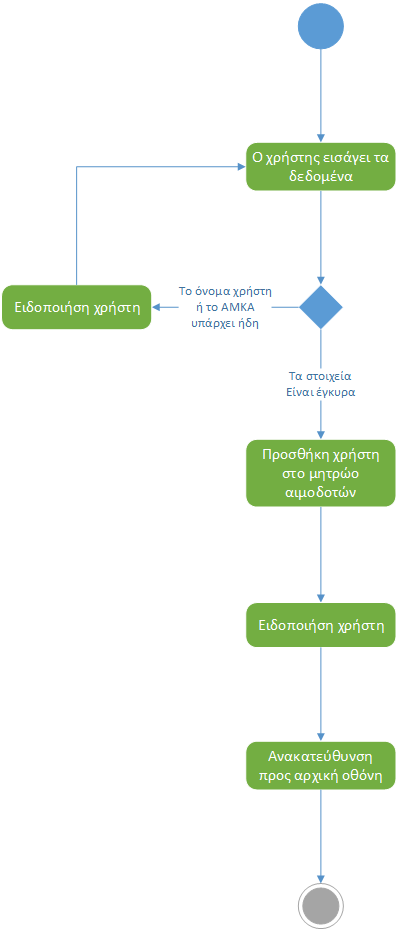
\includegraphics[width=0.7\textwidth]{Register.png}
		    \caption{Ακολουθιακό διάγραμμα \#1. Εγγραφή εθελοντή αιμοδότη στο σύστημα.}
		    \label{fig:register}
		\end{figure}
		
		
		\begin{figure}[H]
		    \centering
		    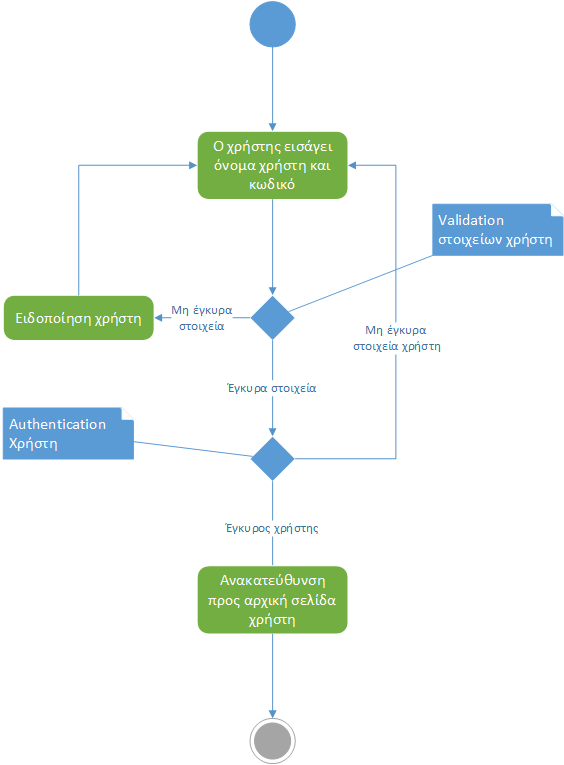
\includegraphics[width=1\textwidth]{Login.png}
		    \caption{Ακολουθιακό διάγραμμα \#2. Είσοδος εθελοντή αιμοδότη στο σύστημα.}
		    \label{fig:login}
		\end{figure}
		
		\begin{figure}[H]
		    \centering
		    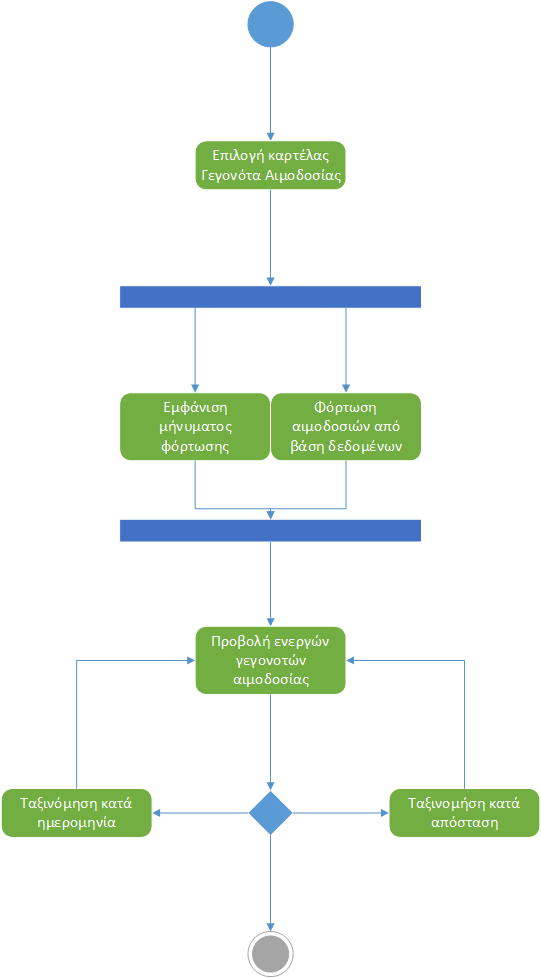
\includegraphics[width=0.7\textwidth]{ViewDonationEvents.png}
		    \caption{Ακολουθιακό διάγραμμα \#3. Προβολή γεγονότων αιμοδοσίας, από τον εθελοντή αιμοδότη.}
		    \label{fig:view}
		\end{figure}
		
	    \begin{figure}[H]
		    \centering
		    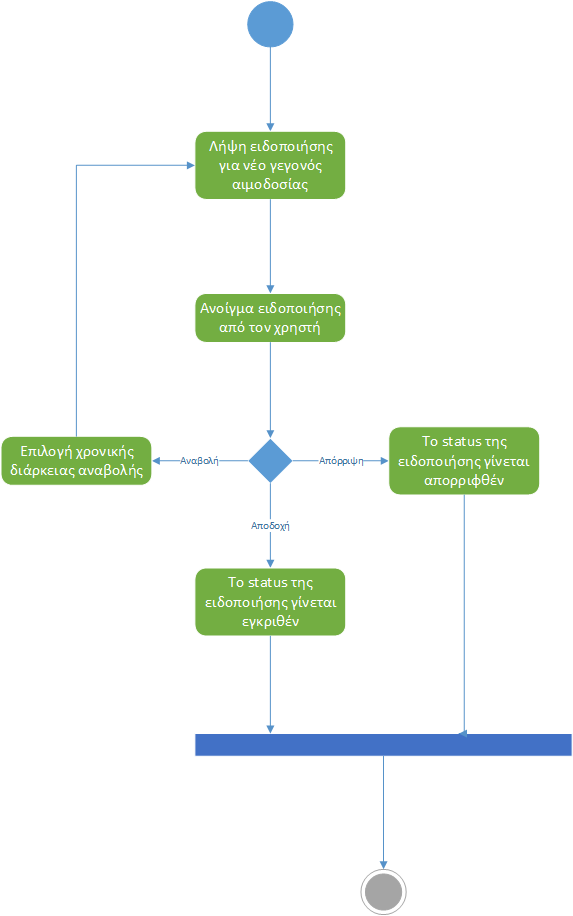
\includegraphics[width=0.9\textwidth]{ManageNotifications.png}
		    \caption{Ακολουθιακό διάγραμμα \#4. Διαχείριση των ειδοποιήσεων για τα γεγονότα αιμοδοσίας από τον εθελοντή αιμοδότη.}
		    \label{fig:manage}
		\end{figure}

		
		\begin{figure}[H]
		    \centering
		    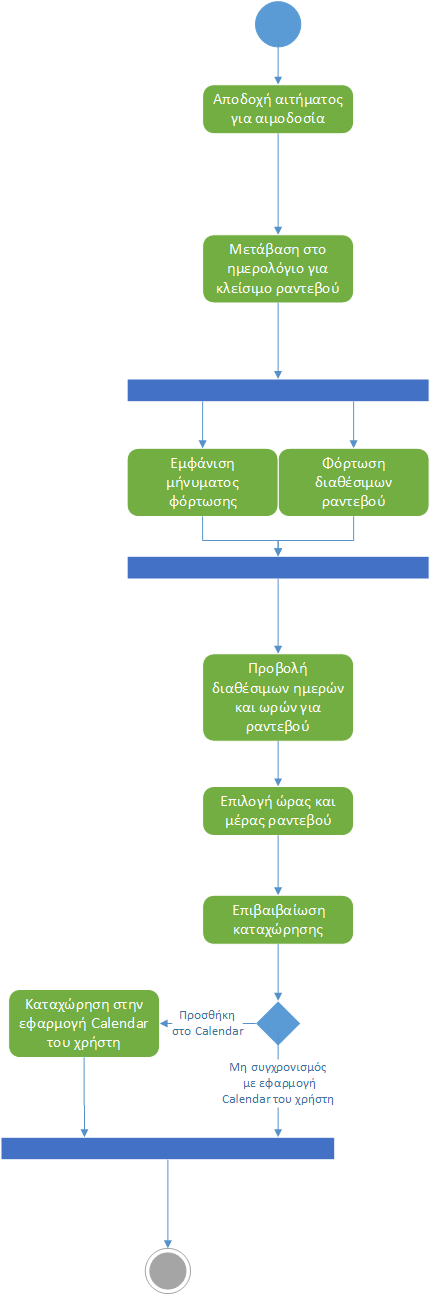
\includegraphics[width=0.5\textwidth]{CreateReservation.png}
		    \caption{Ακολουθιακό διάγραμμα \#5. Κλείσιμο ραντεβού για αιμοδοσία από τον εθελοντή αιμοδότη.}
		    \label{fig:createAppoint}
		\end{figure}
		
				
		\begin{figure}[H]
		    \centering
		    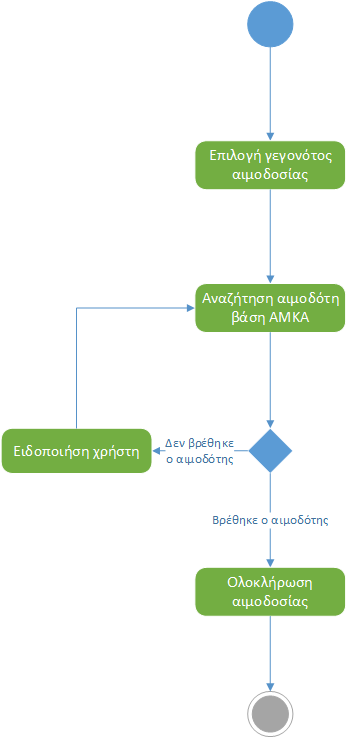
\includegraphics[width=0.7\textwidth]{CompleteDonation.png}
		    \caption{Ακολουθιακό διάγραμμα \#6. Καταχώρηση αιμοδοσίας από τον  εγκεκριμένο χρήστη/διαχειριστή του συστήματος αιμοδοσίας σύστημα.}
		    \label{fig:complete}
		\end{figure}
		
	    \begin{figure}[H]
		    \centering
		    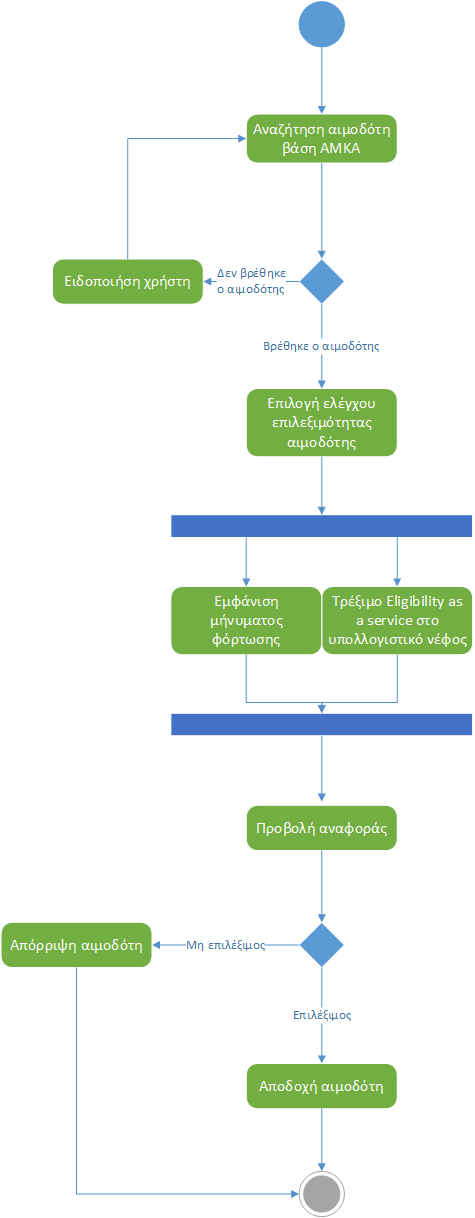
\includegraphics[width=0.55\textwidth]{EligibilityTest.png}
		    \caption{Ακολουθιακό διάγραμμα \#7. Έλεγχος καταλληλότητας του υποψήφιου αιμοδότη από τον  εγκεκριμένο χρήστη/διαχειριστή του συστήματος αιμοδοσίας.}
		    \label{fig:eligibiity}
		\end{figure}
		
\section{Business Model}
	\subsection{Gamification}
	
		Το gamification (παιχνιδοποιήση) ορίζεται ως ``η ενσωμάτωση διάφορων πρακτικών και διαδικασιών παιχνιδιού σε καταστάσεις που δεν σχετίζονται με το παιχνίδι με στόχο τη λύση προβλημάτων μέσω της αύξησης της διαδραστικότητας και της συμμετοχής των χρηστών"\cite{Deterding:2011:GDE:2181037.2181040}\cite{Rojas:2013:MPG:2583008.2583033}. Ως εκ τούτου, το gamification έχει βρει χρήση σε ένα ευρύ φάσμα εφαρμογών, από τον χώρο του marketing και της εκπαίδευσης μέχρι και τον χώρο της υγείας \cite{6758978}. Το Gartner έχει εκτιμήσει ότι μέχρι το τέλος του 2015 περισσότερο από το 50\% των επιχειρήσεων θα αξιοποιεί το gamification \cite{gartnerGamification}. Στον ακαδημαϊκό χώρο συναντάμε όλο και περισσότερη έρευνα και δημοσιεύσεις με στόχο να μελετηθεί με μετρήσιμα, αντικειμενικά κριτήρια κατά πόσο είναι αποτελεσματική η χρήση των τεχνικών gamification. 

	\subsubsection{Δομικά στοιχεία}
	Ένα παιχνίδι αποτελείται από έξι δομικά στοιχεία, όπως παρουσιάζονται στο σχήμα \ref{fig:gamification_components}.
		
		\begin{figure}[h]
		    \centering
		    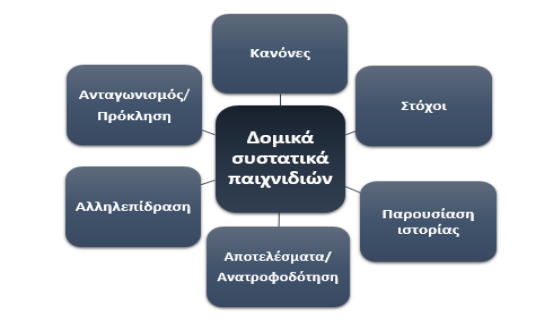
\includegraphics[width=0.7\textwidth]{gamification_components.jpg}
		    \caption{Δομικά στοιχεία παιχνιδιών}
		    \label{fig:gamification_components}
		\end{figure}
	
		Ένας από τους βασικούς στόχους ενός συστήματος gamification αποτελεί η αύξηση της ενασχόλησης του χρήστη. Τα στάδια με τα οποία ευελπιστεί να το πετύχει έχουν ως εξής:
		\begin{enumerate}
			\item Κίνητρα: Στην αρχή της διαδικασίας θα πρέπει να δοθεί στον χρήστη κάποιο κίνητρο το οποίο διαφέρει ανάλογα με τον τύπο χρήστη καθώς και τους στόχους του συστήματος. Παράδειγμα ενός τέτοιου κινήτρου αποτελεί η κοινωνική αναγνώριση \cite{Gamification_on_Participation}.
			\item Ενέργειες: είναι το δεύτερο στάδιο στο οποίο ο χρήστης οδηγείται μέσω των κινήτρων του πρώτου σταδίου. Σε αυτό το στάδιο ο χρήστης πραγματοποιεί την επιθυμητή από το σύστημα ενέργεια. Για παράδειγμα σε μια εφαρμογή εκμάθησης ξένων γλωσσών μια ενέργεια μπορεί να είναι η επανάληψη του λεξιλογίου.
			\item Επιβραβεύσεις: Ύστερα από την επιτυχή ολοκλήρωσης της ενέργειας ή των ενεργειών στο δεύτερο βήμα ο χρήστης λαμβάνει κάποια μορφή επιβράβευσης. Παραδείγματα επιβραβεύσεων που βρίσκουν ευρεία χρήση στο gamification αποτελούν τα εικονικά νομίσματα και τα εικονικά αγαθά.
			\item Κατορθώματα: Στο τελευταίο αυτό στάδιο ο χρήστης φτάνει σε κάποιο κατόρθωμα το οποίο ενισχύει τα κίνητρα του και ο κύκλος επαναλαμβάνεται \cite{GamificationDesign}.
		\end{enumerate}
		Η διαδικασία όπως την περιγράψαμε εμφανίζεται στο σχήμα \ref{fig:engagement_loop}.
		\begin{figure}[h]
		    \centering
		    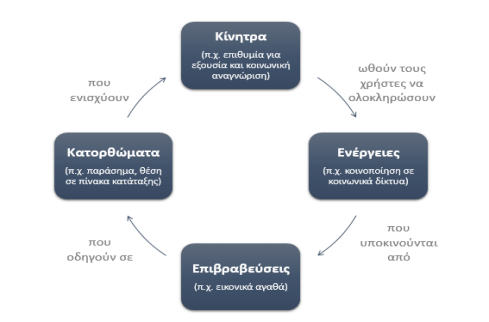
\includegraphics[width=0.7\textwidth]{engagement_loop.jpg}
		    \caption{Κύκλος ενασχόλησης}
		    \label{fig:engagement_loop}
		\end{figure}

	
	\subsubsection{Σχεδιασμός συστήματος}	
		Κατά τον σχεδιασμό του συστήματος gamification ακολουθήσαμε το πλαίσιο ΜΔΑ (MDA), το οποίο προέρχεται από τα αρχικά των λέξεων Μηχανισμοί (Mechanics), Δυναμικές (Dynamics) και Αισθητικά στοιχεία (Aesthetics) \cite{citeulike:382810}. Σύμφωνα με το προαναφερθέν πλαίσιο τα βασικά στοιχεία που απαρτίζουν ένα παιχνίδι είναι οι κανόνες το σύστημα και η διασκέδαση όπως φαίνεται και στο σχήμα \ref{fig:mda_1}.
	
		\begin{figure}[h]
		    \centering
		    
\includegraphics[width=0.7\textwidth]{mda_1.jpg}
		    \caption{Στοιχεία παιχνιδιού}
		    \label{fig:mda_1}
		\end{figure}	
	
		Ενώ για το κομμάτι του σχεδιασμού έχουμε το σχήμα \ref{fig:mda_2}:	
	
		\begin{figure}[h]
		    \centering
		    
\includegraphics[width=0.7\textwidth]{mda_2.jpg}
		    \caption{Πλαίσιο σχεδίασης}
		    \label{fig:mda_2}
		\end{figure}
	
		Πριν προχωρήσουμε στην ανάλυση και παρουσίαση των σχεδιαστικών αποφάσεων που πήραμε, με σκοπό να γίνουν καλύτερα κατανοητές, κρίνουμε σκόπιμο να αναλύσουμε τις παραπάνω έννοιες δεδομένου ότι αποτελεί πολύ συχνό φαινόμενο η ύπαρξη σύγχυσης μεταξύ των εννοιών μηχανισμοί και δυναμικές.
		\begin{itemize}
		
			\item \textbf{Μηχανισμοί:} περιγραφούν συγκεκριμένα δομικά στοιχεία του παιχνιδιού σε επίπεδο αναπαράστασης δεδομένων και αλγορίθμων. Συνδυάζοντας διάφορους βασικούς μηχανισμούς μπορούμε να κατασκευάσουμε πιο πολύπλοκες δομές οι οποίες μπορούν να φέρουν το επιθυμητό αποτέλεσμα. Οι μηχανισμοί είναι αυτοί που υποστηρίζουν τις δυναμικές.
			
			\item \textbf{Δυναμικές:} περιγράφουν πως οι κανόνες του παιχνιδιού αλληλεπιδρούν με τον χρήστη και τους μηχανισμούς. Σε προγραμματιστική ορολογία μπορεί να περιγραφεί ως η συμπεριφορά του παιχνιδιού κατά την διάρκεια εκτέλεσης του. Ρόλος των δυναμικών είναι να κάνουν το παιχνίδι προοδευτικά δυσκολότερο αποφεύγοντας την ρουτίνα και διατηρώντας αμείωτο το ενδιαφέρων του χρήστη.
			\item \textbf{Αισθητικά στοιχεία:} περιγράφουν τα συναισθήματα που επιδιώκει το σύστημα να προξενήσει στον χρήστη του. Σύμφωνα με τους δημιουργούς του προτύπου MDA κάποια από αυτά είναι:
			
			\begin{itemize}
				\item Αίσθηση ( Το παιχνίδι παρουσιάζεται σαν εσωτερική ευχαρίστηση).
				\item Φαντασία (Το παιχνίδι σαν ιστορία με σκοπό να ταξιδέψει τον παίχτη μακριά από την πραγματικότητα).
				\item Αφήγηση (Το παιχνίδι ως ιστορία με πλοκή).
				\item Πρόκληση (Ο παίκτης πρέπει να ξεπεράσει κάποια εμπόδια).
				\item Συνεργασία (Το παιχνίδι με την κοινωνική του υπόσταση).
				\item Ανακάλυψη (Το παιχνίδι με κέντρο την ανακάλυψη του καινούριου).
				\item Έκφραση (Το παιχνίδι ως εξερεύνηση του εαυτού).
				\item Υποβολή (Το παιχνίδι ως απλό μέσο για αναψυχή κατά τον ελέυθερο χρόνο
	του ατόμου).
	
			\end{itemize}
		\end{itemize}
		
		Κατά τον σχεδιασμό ενός συστήματος gamification, λαμβάνοντας υπόψιν τους στόχους του συστήματος γίνεται διαφορετικός συνδυασμός των παραπάνω στοιχείων. Οι πιο συχνά χρησιμοποιούμενοι μηχανισμοί είναι οι πόντοι, οι πίνακες κατάταξης καθώς και τα παράσημα. Στον πίνακα \ref{tab:gamifaction_mechanisms} βλέπουμε διάφορους μηχανισμούς καθώς και τους στόχους που θέλουν να πετύχουν \cite{raey}\cite{Lucassen2014194}.
	
	\begin{table}[H]
		\begin{center}
		    \begin{tabular}{|c|l|}
		    \hline
		    \rowcolor{grayy}
		    \textbf{Στόχος} & \textbf{Μηχανισμός}
		    \\ \hline    
		    \multirow{12}{*}{\textbf{Ενασχόληση}} & Πίνακες Κατάταξης \\ & Επίπεδα \\ & Εικονικές επιβραβεύσεις προσπάθειας \\ & Ανταγωνισμός \\ & Αίσθηση συμμετοχής σε ομάδα \\ &  Έλεγχος σε συμπαίκτες \\ &  Διαφοροποίηση από συμπαίκτες \\ & Βοήθεια σε φίλο \\ & Χρονικοί περιορισμοί \\ & Λήξη χρόνου \\ & Περιορισμοί σε πόρους \\ \hline
		    \multirow{3}{*}{\textbf{Αφοσίωση}}  & Περιορισμοί σε πρόσβαση \\ & Παράσημα \\ & Εικονικές επιβραβεύσεις \\ \hline
		    \multirow{3}{*}{\textbf{Επίγνωση}}  & Προωθήσεις \\ & Λοταρίες  \\ \hline
		    \end{tabular}
		    \caption{Στόχοι και μηχανισμοί του Gamification}
			\label{tab:gamifaction_mechanisms}
		\end{center}
	\end{table}

		Για να γίνει ξεκάθαρος ο διαχωρισμός μεταξύ δυναμικών και μηχανισμών στον πίνακα \ref{tab:gamifaction_dynamics} παρουσιάζουμε τους μηχανισμούς ενός παιχνιδιού με τις αντίστοιχες δυναμικές και κίνητρα \cite{BlohmIvo2013}.
	
	\begin{table}[H]
		\begin{center}
		    \begin{tabular}{|l|l|l|}
		    \hline
		    \rowcolor{grayy}
		    \textbf{Μηχανισμοί} & \textbf{Δυναμικές} & \textbf{Κίνητρα}
		    \\ \hline
		     Καταγραφή συμπεριφοράς & Εξερεύνηση & Περιέργεια   
		     \\ \hline
		     Συστήματα πόντων, εμβλήματα και επιβραβεύσεις & Συλλογή (εικονικών αγαθών) & Κατόρθωμα
		     \\ \hline
		     Κατάταξη, επίπεδα & Ανταγωνισμός & Κοινωνική αναγνώριση
		     \\ \hline
		     Ομαδικές δραστηριότητες & Συνεργασία & Επικοινωνία
		     \\ \hline
		     Πίεση χρόνου, χρονική περιορισμοί & Πρόκληση & Διέγερση
		     \\ \hline
		     Εικονικοί χαρακτήρες και κόσμοι & Ανάπτυξη, Οργάνωση & Αυτοδιάθεση
		     \\ \hline
		    \end{tabular}
		    \caption{Μηχανισμοί, δυναμικές και κίνητρα στο Gamification}
			\label{tab:gamifaction_dynamics}
		\end{center}
	\end{table}
	
	\subsubsection{Gamification στο σύστημα μας}
		Έχοντας παρουσιάσει το θεωρητικό πλαίσιο του gamification, στην συνέχεια παρουσιάζουμε την χρήση του στο σύστημα που αναπτύξαμε στο πλαίσιο της παρούσας διπλωματικής. Μέσω του gamification επιδιώκουμε να πετύχουμε κυρίως τους δύο πρώτους στόχους της διπλωματικής όπως περιγράφηκαν στην ενότητα \ref{sec:intro_goals}.
		
	\subsubsection{Σύστημα επιβραβεύσεων}
	Οι επιβραβεύσεις δίνονται στον εθελοντή αιμοδότη (χρήστη του συστήματος) ανάλογα με την δραστηριότητα του και τους πόντους που έχει συγκεντρώσει. Οι επιβραβεύσεις μπορούν να χωριστούν σε δύο μεγάλες κατηγορίες:
	\begin{itemize}
		\item \textbf{Φυσικές Επιβραβεύσεις:} Ο χρήστης θα μπορεί να εξαργυρώνει τους πόντους που έχει μαζέψει για να κερδίσει υπηρεσίες ή προϊόντα από συνεργαζόμενες υπηρεσίες που τα έχουν διαθέσει τα πλαίσια κοινωνικής ευθύνης. Για παράδειγμα αν υπάρξει κάποια συνεργασία με την Cosmote μια μορφή φυσικής επιβράβευσης θα μπορούσε να είναι επιπλέον χρόνος ομιλίας.
		 \item \textbf{Εικονικές Επιβραβεύσεις:} Η μορφή των εικονικών επιβραβεύσεων που χρησιμοποιήσαμε στο σύστημα μας είναι τα εμβλήματα, τα οποία ο χρήστης θα λαμβάνει για διάφορες δραστηριότητες που επιτελεί. Συγκεκριμένα ο χρήστης κερδίζει εμβλήματα όταν:
		 
		 	\begin{itemize}
		 		\item Εγγράφεται στο σύστημα ως εθελοντής αιμοδότης
		 		\item Πραγματοποιεί την πρώτη του αιμοδοσία
		 		\item Συμπληρώνει τον μέγιστο αριθμό αιμοδοσιών που επιτρέπεται σε κάποιο ημερολογιακό έτος
		 		\item Καλεί κάποιον φίλο του να χρησιμοποιήσει την εφαρμογή
		 		\item Ανταποκρίνεται σε αιτήματα για αιμοδοσίες
		 	\end{itemize}
		 	Η παραπάνω λίστα είναι καθαρά ενδεικτική, δεδομένου ότι η δημιουργία εμβλημάτων αποτελεί μια δυναμική διαδικασία που έχει σκοπό να κρατήσει αμείωτο το ενδιαφέρον του εθελοντή. Για παράδειγμα ο διαχειριστής του συστήματος θα μπορεί να δημιουργεί ειδικά εμβλήματα για ένα συγκεκριμένο γεγονός αιμοδοσίας το οποίο έχει συγκεκριμένη ημερομηνία.
	\end{itemize}
	
	Σε αυτό το σημείο θα πρέπει να αναφέρουμε ότι, έχει αποτελέσει αντικείμενο τεράστιας διαμάχης το κατά πόσο πρέπει να δίνονται φυσικές επιβραβεύσεις στους εθελοντές και κατά πόσο αυτό αφαιρεί το νόημα της εθελοντικής αιμοδοσίας. Στην Ελλάδα μέχρι πρωτινός δεν επιτρεπόντουσαν κίνητρα που θα μπορούσαν να θεωρηθούν αντικαταστατό του χρήματος, αλλά ο πρόσφατος νόμος 4272/2014 άρθρο 27 δίνει την ελευθερία στον Ε.ΚΕ.Α. να ορίσει τέτοιου είδους κίνητρα σε συμφωνία με την οδηγία 2002/98 της Ευρωπαϊκής ένωσης.
	
	\subsubsection{Σύστημα πόντων}\label{sssect:point_system}
	
	Το σύστημα gamification που εφαρμόζουμε στην εφαρμογή που αναπτύχθηκε στα πλαίσια της παρούσας διπλωματικής περιλαμβάνει ολοκληρωμένο σύστημα πόντων. Ο χρήστης με το που εγγράφεται στο σύστημα λαμβάνει έναν μικρό αριθμό πόντων ως επιβράβευση της εγγραφής του ως εθελοντής αιμοδότης. Οι πόντοι μπορούν αν χωριστούν σε δύο επιμέρους κατηγορίες βάση της χρήσης τους:

	\begin{itemize}
		\item \textbf{Πόντοι εξαργύρωσης:} εξαργυρώνονται με σκοπό της απόκτησης κάποιας επιβράβευσης. Ανάλογα με τις δραστηριότητες που επιτελεί κερδίζει πόντους οι οποίοι αθροίζονται. Ενδεικτική λίστα για τις οποίες ο χρήστης θα μπορεί να κερδίζει πόντους:
		\begin{itemize}
			\item Εγγραφή στο σύστημα.
			\item Πραγματοποίηση αιμοδοσίας.
			\item Πρόσκληση φίλων στην εφαρμογή.
			\item Αλληλεπίδραση με τα κοινωνικά δίκτυα.
		\end{itemize}
		\item \textbf{Πόντοι εμπειρίας:} ουσιαστικά είναι οι συνολικοί πόντοι που έχει αποκτήσει ο εθελοντής από την έναρξη χρήσης της εφαρμογής. Οι πόντοι εμπειρίας χρησιμοποιούνται για τον πίνακα κατάταξης μεταξύ των ``φίλων" του, καθώς και για τον συνολικό πίνακα κατάταξης.
	\end{itemize}
	Κρίνεται σκόπιμο να αναφερθεί ότι οι πόντοι κατανέμονται με βάση την βαρύτητα της δραστηριότητας που εκτελεί ο εθελοντής αιμοδότης.
	
	\subsubsection{Πίνακες κατάταξης}
	
	Οι πίνακες κατάταξης δείχνουν την επίδοση και την `πρόοδο' ενός χρήστη σε σχέση με αυτή των `φίλων' τους \cite{Liu:2011:GIE:2072652.2072655}. Υπάρχει ένας ενιαίος πίνακας στον οποίο και θα υπάρχουν όλοι οι εθελοντές που χρησιμοποιούν το σύστημα, εφόσον έχουν δηλώσει ότι επιθυμούν να συμμετέχουν στην κατάταξη. Ενώ υπάρχει και ένας δεύτερος πίνακας που δημιουργείται δυναμικά για κάθε χρήστη και περιλαμβάνει μόνο άτομα τα οποία ακολουθεί. Η κατάταξη διαμορφώνεται με βάση τους πόντους εμπειρίας που έχει μαζέψει κάθε χρήστης, οι οποίοι περιγράφηκαν παραπάνω. Για τους πρώτους στον κεντρικό πίνακα κατάταξης θα υπάρχει μέριμνα για κάποια ειδική επιβράβευση, ανάλογα τις συμφωνίες και χορηγίες που υπάρχουν με εταιρείες στα πλαίσια της κοινωνικής ευθύνης.
	
	\subsubsection{Συμπέρασμα}
	
	Συμπερασματικά το σύστημα που περιγράψαμε παραπάνω μπορεί να βοηθήσει σημαντικά στον δεύτερο στόχο που θέσαμε στην εισαγωγή της διπλωματικής, στην ενότητα \ref{sec:intro_goals}, δηλαδή στη διατήρηση και επιπλέον ενεργοποίηση των εθελοντών αιμοδοτών. Για την επίτευξη του πρώτου στόχου που θέσαμε δηλαδή τη στρατολόγηση περισσότερων νέων εθελοντών θεωρούμε πως μεγάλο ρόλο μπορεί να παίξει ο συνδυασμός του gamification με τα κοινωνικά δίκτυα όπως περιγράφουμε στην επόμενη ενότητα.
	
	\subsection{Social Networking Integration}\label{ssec:social_netowrks_system_analysis}

	Η θεωρία της κοινωνικοποίησης των καταναλωτών προβλέπει ότι η επικοινωνία μεταξύ των καταναλωτών επηρεάζει τη γνωστική και συναισθηματική τους συμπεριφορά, καθώς και τις στάσεις τους απέναντι σε ένα προϊόν ή μια υπηρεσία\cite{1974}. Τα κοινωνικά δίκτυα μπορούν να επηρεάσουν δραστικά την συμπεριφορά ενός ατόμου\cite{shaver2007impact} και οι υπάρχοντες εθελοντές μέσω των κοινωνικών δικτύων, είναι σε θέση να παίξουν τον ρόλο του πρέσβη προσελκύοντας νέους εθελοντές αιμοδότες. Η αξιοποίηση των εθελοντών με στόχο την προαγωγή της εθελοντικής αιμοδοσίας, αποτελεί μια εξαιρετικά αποτελεσματική μέθοδο "στρατολόγησης" και αύξησης του αριθμού των αιμοδοσιών \cite{Lemmens2008}. Πριν προχωρήσουμε στην ανάλυση των συγκεκριμένων ενεργειών που επιτελέσαμε με αυτό τον σκοπό, κρίνουμε σκόπιμο να αναφέρουμε μερικές εισαγωγικές έννοιες για τα κοινωνικά δίκτυα εν γένει. 	
	
	Τα μέσα κοινωνικής δικτύωσης (Social Media), μέσω των οποίων επιτυγχάνεται η ηλεκτρονική κοινωνική δικτύωση, αποτελούν ουσιαστικά απόρροια του Web 2.0, το οποίο κατάφερε να αλλάξει την υφή του διαδικτύου προσδίδοντάς του μια πιο κοινωνική διάσταση. Ο όρος κοινωνικά δίκτυα (social media), αποτελεί μια γενική έννοια που χρησιμοποιείται για να περιγράψει διαδικτυακές εφαρμογές και υπηρεσίες στις οποίες οι χρήστες έχουν την δυνατότητα να δημιουργήσουν και να μοιραστούν μεταξύ τους περιεχόμενο \cite{Kaplan201059}. Τα μέσα κοινωνικής δικτύωσης μπορούν να χωριστούν σε έξι κατηγορίες με βάση τον βαθμό της κοινωνικής παρουσίας που απαιτούν από τον χρήστη:
	\begin{itemize}
		\item Ιστολόγια (π.χ Blogger, Tumblr, Wordpress)
		\item Συνεργατικές ιστοσελίδες - έργα (π.χ Wikipedia)
		\item Ιστοσελίδες κοινωνικής δικτύωσης (π.χ Facebook)
		\item Κοινότητες διαμοιρασμού περιεχομένου (π.χ Reddit, Youtube)
		\item Εικονικοί κόσμοι (π.χ Second Life)
		\item Εικονικοί κόσμοι παιχνιδιών (π.χ World of Warcraft)
	\end{itemize}
	
	Τα μέσα κοινωνικής δικτύωσης βρήκαν τέτοια ευρεία αποδοχή και εδραιώθηκαν στην καθημερινότητα μας γιατί ικανοποιούν μια ισχυρή ανάγκη του ανθρώπου. Την ανάγκη του να συνεταιρίζεται, δημιουργώντας δίκτυα με άλλους ανθρώπους, ανταλλάζοντας ιδέες και απόψεις. Τα κύρια κίνητρα για τη χρήση των μέσων κοινωνικής δικτύωσης είναι τα εξής \cite{Benkler2006}:
	\begin{itemize}
		\item Κοινωνικοποίηση
		\item Ψυχική ευεξία
		\item Ατομική ικανοποίηση
		\item Κοινωνική αναγνώριση
	\end{itemize}		
	
	Όπως αναφέραμε και παραπάνω ο κύκλος της ενασχόλησης (σχήμα \ref{fig:engagement_loop}) ξεκινάει από το κίνητρο. Ένα από τα βασικότερα κίνητρα του ανθρώπου είναι η επιθυμία για κοινωνική αναγνώριση και προβολή \cite{Gamification_on_Participation} την οποία πολλές φορές επιδιώκει να ικανοποιήσει μέσω των κοινωνικών δικτύων (όπως φαίνεται από την παραπάνω λίστα).
	
	Η εφαρμογή που αναπτύξαμε στα πλαίσια της διπλωματικής εργασίας δίνει την δυνατότητα στον εθελοντή (χρήστη) να μοιραστεί στα κοινωνικά δίκτυα τα επιτεύγματα του καθώς και πληροφορίες σε κάθε στάδιο της αιμοδοσίας, ικανοποιώντας με αυτό τον τρόπο το αίσθημα της κοινωνικής αναγνώρισης. Συγκεκριμένα υπάρχει άμεση διασύνδεση με το facebook και το twitter στα οποία ο χρήστης ενθαρρύνεται να δημοσιεύσει στις παρακάτω περιπτώσεις:
	\begin{itemize}
		\item Όταν λαμβάνει ειδοποίηση για γεγονός αιμοδοσίας, του δίνεται η δυνατότητα να το μοιραστεί στα μέσα κοινωνικής δικτύωσης. Με αυτό τον τρόπο αυξάνεται η προβολή του γεγονότος αιμοδοσίας και κατ' επέκταση οι πιθανότητες να καλυφθούν οι ανάγκες σε αίμα που έχουν τεθεί, ενώ προβάλλεται και η ίδια η εφαρμογή το οποίο οδηγεί στην στρατολόγηση περισσότερων εθελοντών αιμοδοτών.
		\item Όταν ολοκληρώνει κάποια αιμοδοσία ο χρήστης παροτρύνεται να βγάλει φωτογραφία και να τη μοιραστεί στα μέσα κοινωνικής δικτύωσης, προάγοντας την αιμοδοσία.
		\item Όταν ξεκλειδώνει κάποιο έμβλημα.
	\end{itemize}
	
	Επίσης ο χρήστης έχει τη δυνατότητα να προσκαλέσει τους φίλους του στην εφαρμογή. Σε αυτό το σημείο πρέπει να αναφερθεί ότι κάθε φορά που ο χρήστης αλληλεπιδρά μέσω της εφαρμογής με τα μέσα κοινωνικής δικτύωσης κερδίζει πόντους σύμφωνα με το σύστημα πόντων όπως περιγράφηκε στο \ref{sssect:point_system} . Αξιοποιώντας τη δύναμη των κοινωνικών δικτύων είμαστε σε θέση να δώσουμε μεγαλύτερη προβολή και κοινωνικό χαρακτήρα στην εθελοντική αιμοδοσία. Μετατρέποντας ουσιαστικά τους εθελοντές αιμοδότες σε πρότυπα της εθελοντικής αιμοδοσίας με στόχο την προσέλκυση νέων εθελοντών αιμοδοτών.
	
	\subsection{Ειδοποιήσεις και Υπενθυμίσεις}
		
		 Όταν υπάρχει κάποια συγκεκριμένη ανάγκη για αίμα ή ένα καθορισμένο γεγονός αιμοδοσίας, το σύστημα στέλνει στους εθελοντές αιμοδότες νέες ειδοποιήσεις (push notifications). Οι ειδοποιήσεις αυτές δεν αποστέλλονται σε όλους τους χρήστες που είναι εγγεγραμμένοι στην εφαρμογή, αντιθέτως το σύστημα τρέχει κάποιους ``έξυπνους αλγορίθμους" και επιλέγει την ομάδα χρηστών που τηρούν τις απαραίτητες προϋποθέσεις. Τα κριτήρια που ελέγχει το σύστημα αφορούν στο αν έχει παρέλθει το απαιτούμενο διάστημα μέχρι να μπορεί να δώσει ξανά αίμα ο εθελοντής, στην καταλληλότητα με βάση τη γεωγραφική του τοποθεσία και στο αν έχει τη ζητούμενη ομάδα αίματος, στην περίπτωση που υπάρχουν .
		 
		
		Ο χρήστης έχει την επιλογή να αποδεχθεί, να απορρίψει και να αναβάλει την ειδοποίηση. Στην περίπτωση αποδοχής, ο χρήστης μπορεί να κλείσει ένα ραντεβού με το αντίστοιχο κέντρο αιμοδοσίας καθώς το σύστημα παρέχει ολοκληρωμένη διαχείριση ραντεβού. Η εφαρμογή έχει τη δυνατότητα να παρέχει υπενθυμίσεις εγκαίρως μέσα από πολλούς διαφορετικούς τρόπους, όπως μήνυμα ηλεκτρονικού ταχυδρομείου, επαναποστολή της ειδοποίησης και συγχρονισμός και καταχώρηση στο ημερολόγιο του χρήστη). Σε περίπτωση που ο χρήστης απορρίψει ένα αίτημα, αυτό μεταφέρεται και εμφανίζεται αυτόματα στο ιστορικό των χρηστών, στην ενότητα των απορριφθέντων αιτημάτων. Ως εκ τούτου ο χρήστης μπορεί να αναθεωρήσει τα αιτήματα του και να το εξετάσει σε μεταγενέστερο χρόνο. 
		
		 Σύμφωνα με μελέτες που έχουν γίνει υπάρχει μεγάλος αριθμός αιμοδοτών που ενώ πληρούν τις απαραίτητες προϋποθέσεις και έχουν την θέληση να αιμοδοτήσουν, δεν προβαίνουν σε αιμοδοσία επειδή δεν υπάρχει κάποιος να τους το υπενθυμίσει \cite{Marantidou2007}. Η αντιμετώπιση αυτού του προβλήματος επιτυγχάνεται με τις συστηματικές ειδοποιήσεις που λαμβάνει ο αιμοδότης, οι οποίες εκτός από μέσο για υπενθύμιση, δρουν ως κινητήριος δύναμη αφύπνισης και διατήρησης της εθελοντικής συνείδησης του αιμοδότη.
		 
		 Ένα άλλο φαινόμενο το οποίο δυσχεραίνει ακόμα περισσότερο την ήδη δύσκολη κατάσταση στον τομέα των αιμοδοσιών είναι η προσωρινή απόρριψη των αιμοδοτών.  Το φαινόμενο αυτό  λαμβάνει χώρα σε περιπτώσεις που οι χρήστες αποκλείονται προσωρινά από την αιμοδοσία, λόγω του ότι δεν τηρούν τα κριτήρια ακαταλληλότητας (π.χ. πήραν ασπιρίνη την ημέρα της αιμοδοσίας). Από τον συνολικό αριθμό αιμοδοσιών το 14.13\% αποκλείονται για λόγους προσωρινής ακαταλληλότητας \cite{WorldHealth}. Μελέτες έχουν δείξει ότι οι περισσότεροι εθελοντές δεν επιστρέφουν αν απορριφθούν μία φορά, συγκεκριμένα μόλις το 11\% επιστρέφει μετά την απαιτούμενη περίοδο για να πραγματοποιήσει δωρεά αίματος \cite{halperin1998effect}. Όταν τηρούνται οι κατάλληλες συνθήκες ώστε να είναι σε θέση ο αιμοδότης να προσφέρει πάλι αίμα, η εφαρμογή του στέλνει ειδοποιήσεις για τα γεγονότα αιμοδοσίας ώστε να τον παρακινήσει και να του υπενθυμίσει να δώσει αίμα.
		 
	
		 Με βάση τα όσα προαναφέρθηκαν, η χρήση κατάλληλων ειδοποιήσεων και ως προς την χρονική συχνότητα και ως το προς τον παραλήπτη τους, βοηθάει στην τακτική συμμετοχή των εθελοντών σε αιμοδοσίες και συντελεί στην αντιμετώπιση κάποιων από τα προβλήματα που τους αποθαρρύνουν. Η σωστή διαχείριση και αποστολή των ειδοποιήσεων είναι ένα πολύ σημαντικό ζήτημα, καθώς δεν πρέπει να στέλνονται περιττές ή λανθασμένα επαναλαμβανόμενες ειδοποιήσεις, οι οποίες μπορεί να έχουν ως αποτέλεσμα να κουράσουν τον χρήστη αλλά πρέπει η συχνότητα αποστολής τους να αποφέρει το βέλτιστο αποτέλεσμα. Στόχος του συστήματος ειδοποιήσεων είναι η ανταπόκριση να αυξηθεί με ικανοποιητικό ρυθμό και οι αιμοδοσίες να πολλαπλασιαστούν\cite{Marantidou2007}.
	
	
	\subsection{Heamovigilance}
	
		Ένα άλλο θέμα για το οποίο λαμβάνεται μέριμνα είναι το ζήτημα της αιμοεπαγρυπνήσης. Μία απαραίτητη προϋπόθεση για την αποτελεσματική εφαρμογή της αιμοεπαγρυπνήσης είναι η ύπαρξη συστήματος ιχνηλασιμότητας, δηλαδή πρέπει να εξασφαλίζεται η ικανότητα εντοπισμού καθεμίας από τις μονάδας αίματος ή καθενός από τα παράγωγα προϊόντα αίματος που προέρχονται από αυτήν, από τον εθελοντή αιμοδότη μέχρι τον τελικό προορισμό τους.
		
		
		Το σύστημα μας, αρχικά καταγράφει τον αιμοδότη από τον οποίο προήλθε το αίμα. Στην συνέχεια, κάθε μονάδα αίματος παρακολουθείται με χρήση RFIDs και όταν τελικά φτάσει στον τελικό αποδέκτη το πληροφοριακό σύστημα του νοσοκομείου αποθηκεύει την πληροφορία αυτή στο πληροφοριακό του σύστημα. Με χρήση κατάλληλων πρωτοκόλλων και ασφαλούς διαύλου επικοινωνίας το σύστημα μας λαμβάνει από το πληροφοριακό σύστημα του νοσοκομείου το όνομα και το μοναδικό αναγνωριστικό του ασθενούς (ΑΜΚΑ) και τα αποθηκεύει, συσχετίζοντας τα με τα στοιχεία του αιμοδότη. Αυτή η διαδικασία έχει ως αποτέλεσμα να κρατείται πλήρες ηλεκτρονικό αρχείο το οποίο συσχετίζει σε περιπτώσεις ανεπιθύμητων συμβαμάτων τον αιμοδότη με τον αιμολήπτη. Η λειτουργία είναι ιδιαίτερα σημαντική για την ελαχιστοποίηση των ανεπιθύμητων κρουσμάτων και κατ 'επέκταση για τη δημόσια υγεία.	


	